\section{Results}

The aim of this project has been to realize the double Fano cavity experimentally and investigate it's transmission profile as a function of the incident wavelength. In this section I present the best results obtained and comment on these. Furthermore, I will outline challenges and obstacles that have been encountered, their implications on the data presented and my thoughts on immediate improvements for future experiments. 

The results obtained have been so through an iterative process realizing the theory presented in previous sections. For this reason, the structure of this section will outline this process and thus begin by an in depth spectral analysis of the Fano mirrors used, as a pair matching in optical parameters, and especially the guided-mode resonance wavelength, is crucial in order to realize the Fano resonance. When moving on to the results regarding cavity characterization I will begin by briefly verifying the results for the single Fano cavity presented by Mitra et al. in \cite{Mitra}. Finally, I will show experiemental results of the optical characterization of the double Fano cavity. 

\subsection{Fano mirror characterization}\label{sec:results_fano_mirror_characterization}

The first important step in realizing the double Fano cavity, is to locate a matching pair of Fano mirrors, as a substantial spectral overlap is necessary in order to excite a Fano resonance including both guided-modes, as explained in section \ref{sec:spectral_detuning}. For this reason the Fano mirrors considered were all fabricated externally by \emph{Norcada} and furthermore from the same batch, as these were initially considered to have a greater probability of having similar physical attributes. Many Fano mirrors were thus characterized during the process of finding a match, and the pair eventually chosen to move forward with were denoted \emph{G1} and \emph{G2}. 

\begin{figure}[h!]
    \centering
    \begin{subfigure}[b]{0.49\textwidth}
        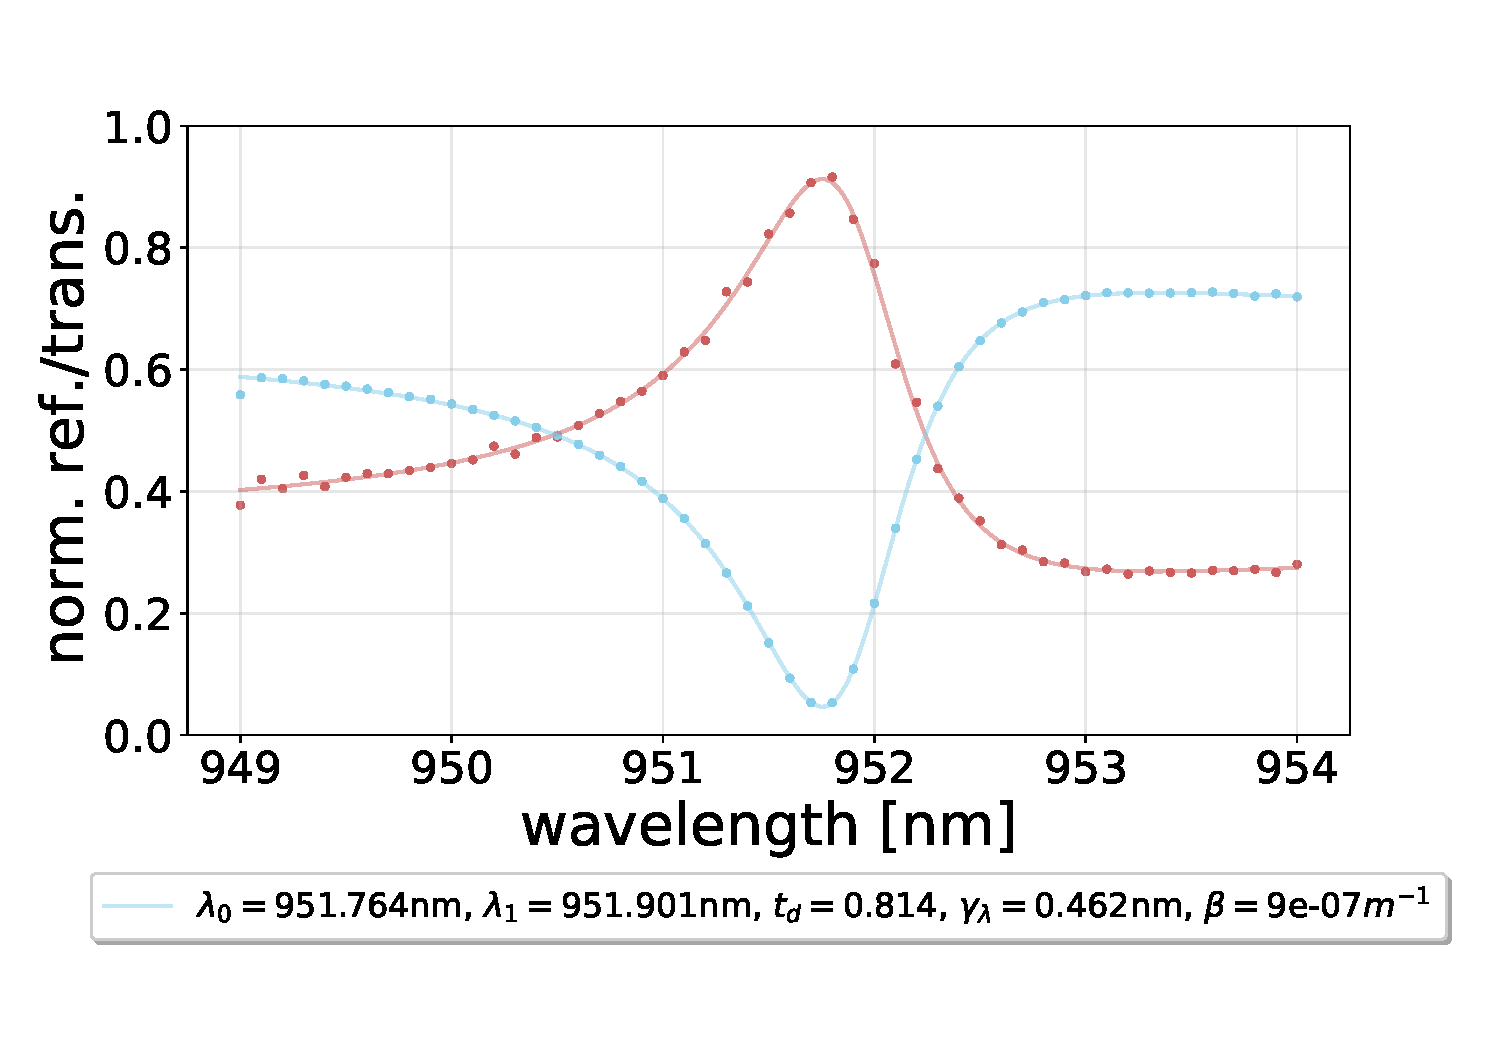
\includegraphics[width=\textwidth]{figures/results/M3:M5/M5:G1_initial_spectrum.pdf}
        \caption{}
        \label{}
    \end{subfigure}
    \begin{subfigure}[b]{0.49\textwidth}
        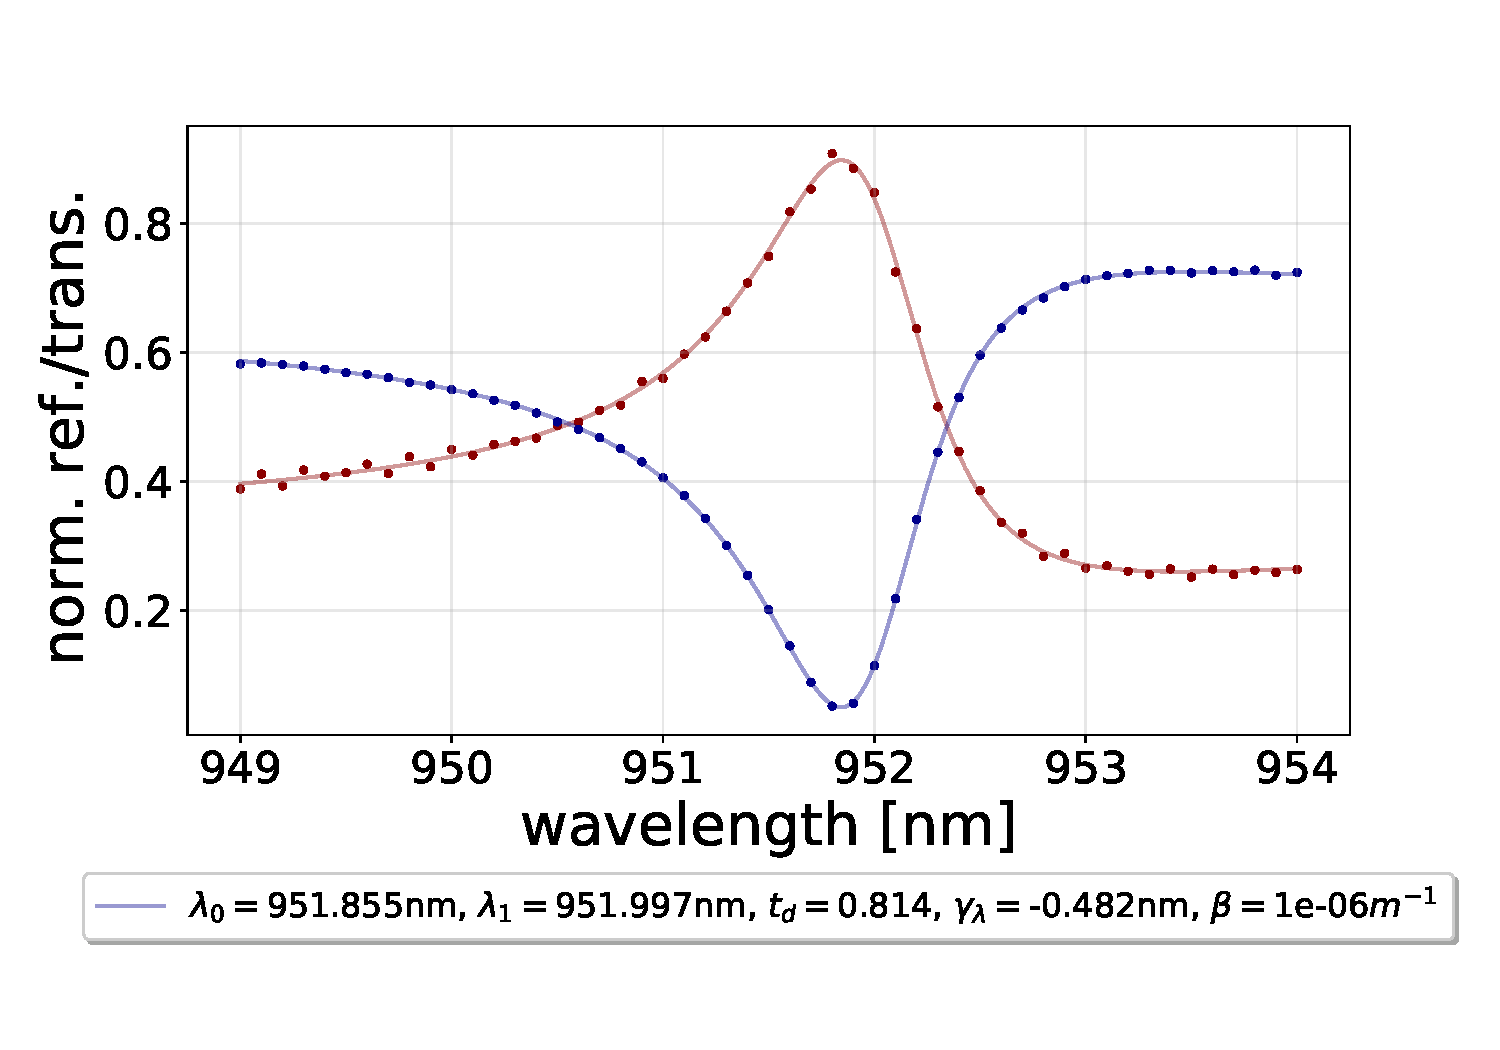
\includegraphics[width=\textwidth]{figures/results/M3:M5/M3:G2_initial_spectrum.pdf}
        \caption{}
        \label{}
    \end{subfigure}
    \caption{}
    \label{fig:individual_G1_and_G2_spectra}
\end{figure}

Figure \ref{fig:individual_G1_and_G2_spectra} show the individual measured normalized reflection and transmission spectra of G1 and G2 together with a least squares fit to the model derived in section \ref{sec:fano_mirror}. The corresponding optical parameters for each Fano mirror were found as the following.

Fitting parameters for G1:
\begin{equation}
    \begin{split}
        \lambda_{0,G1} &= 951.764 \text{nm}, \:\: \lambda_{1,G1} = 951.901 \text{nm},\:\: t_d = 0.814, \\&r_d = 0.575, \:\:  \gamma_{\lambda} = 0.462 \text{nm},\:\: \beta = 9 \cdot 10^{-7} \text{m}^{-1}.
    \end{split}
    \label{eq:G1_params}
\end{equation}

Fitting parameters for G2:
\begin{equation}
    \begin{split}
        \lambda_{0,G2} &= 951.855 \text{nm}, \:\: \lambda_{1,G2} = 951.997 \text{nm},\:\: t_d = 0.814, \\&r_d = 0.570, \:\:  \gamma_{\lambda} = 0.482 \text{nm},\:\: \beta = 1 \cdot 10^{-6} \text{m}^{-1}.
    \end{split}
    \label{eq:G2_params}
\end{equation}

In order to evaluate and compare the parameters to determine whether the two Fano mirrors are in fact a good match, they are both shown alongside eachother in figure \ref{fig:G1_and_G2_spectral_comparison} for spectral comparison. Each their resonance wavelengths $\lambda_0$ are indicated on the figure and the detuning can thus be estimated as 
\begin{equation}
    \Delta = \left|\lambda_{0,G2} - \lambda_{0,G1}\right| = 951.855 \text{nm} - 951.764 \text{nm} = 0.091 \text{nm}.
    \label{eq:G1/G2_detuning}
\end{equation}

Here we remember that the additional fitting parameters, namely $t_d$, $r_d$, $\gamma_{\lambda}$ and $\beta$, are assumed identical in the model for the double Fano cavity outlined in section \ref{sec:double_fano_lw_theory} and these are thus compared in a more qualitative manner. Whether the parameters in eqs. (\ref{eq:G1_params}) and (\ref{eq:G2_params}) can be assumed identical is completely individual to the given experiment and the corresponding acceptable margins. In order to move forward, G1 and G2 are assumed to only differ in guided-mode resonance wavelength.

\begin{figure}[h!]
    \centering
    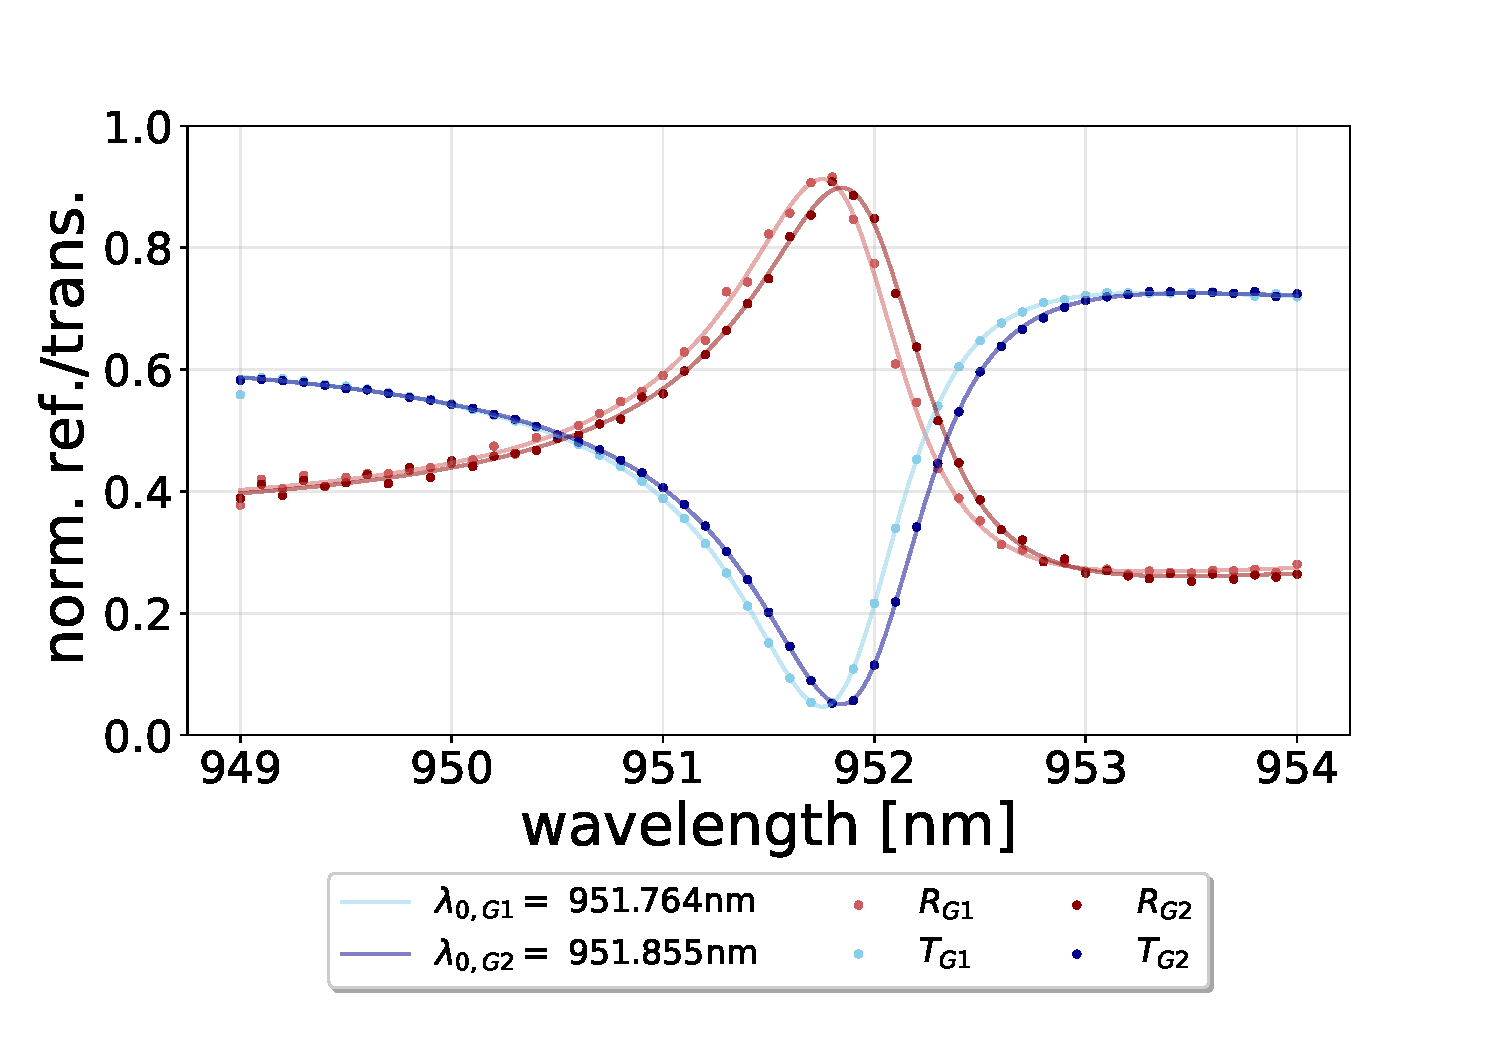
\includegraphics[width=0.7\textwidth]{figures/results/M3:M5/M3:M5_initial_spectra.pdf}
    \caption{}
    \label{fig:G1_and_G2_spectral_comparison}
\end{figure}

As is shown in section \ref{sec:spacial_detuning}, a spectral detuning leads to a spacial detuning, meaning that the cavity length corresponding to the guided-mode resonance wavelength for G1 and G2 are not identical as they have a non-zero detuning $\Delta$. In order to sustain a Fano resonance it is equally important that the Fano mirrors have overlapping cavity transmission profiles as a function of the cavity length. Figure \ref{fig:G1/G2_length_scan} shows the simulated double Fano transmission of a cavity consisting of G1 and G2 for length corresponding to their guided-mode resonance wavelengths. It is readily seen that the two transmission profiles overlap for the included example of a cavity of length $l \approx 30 \mu m$.

\begin{figure}[h!]
    \centering
    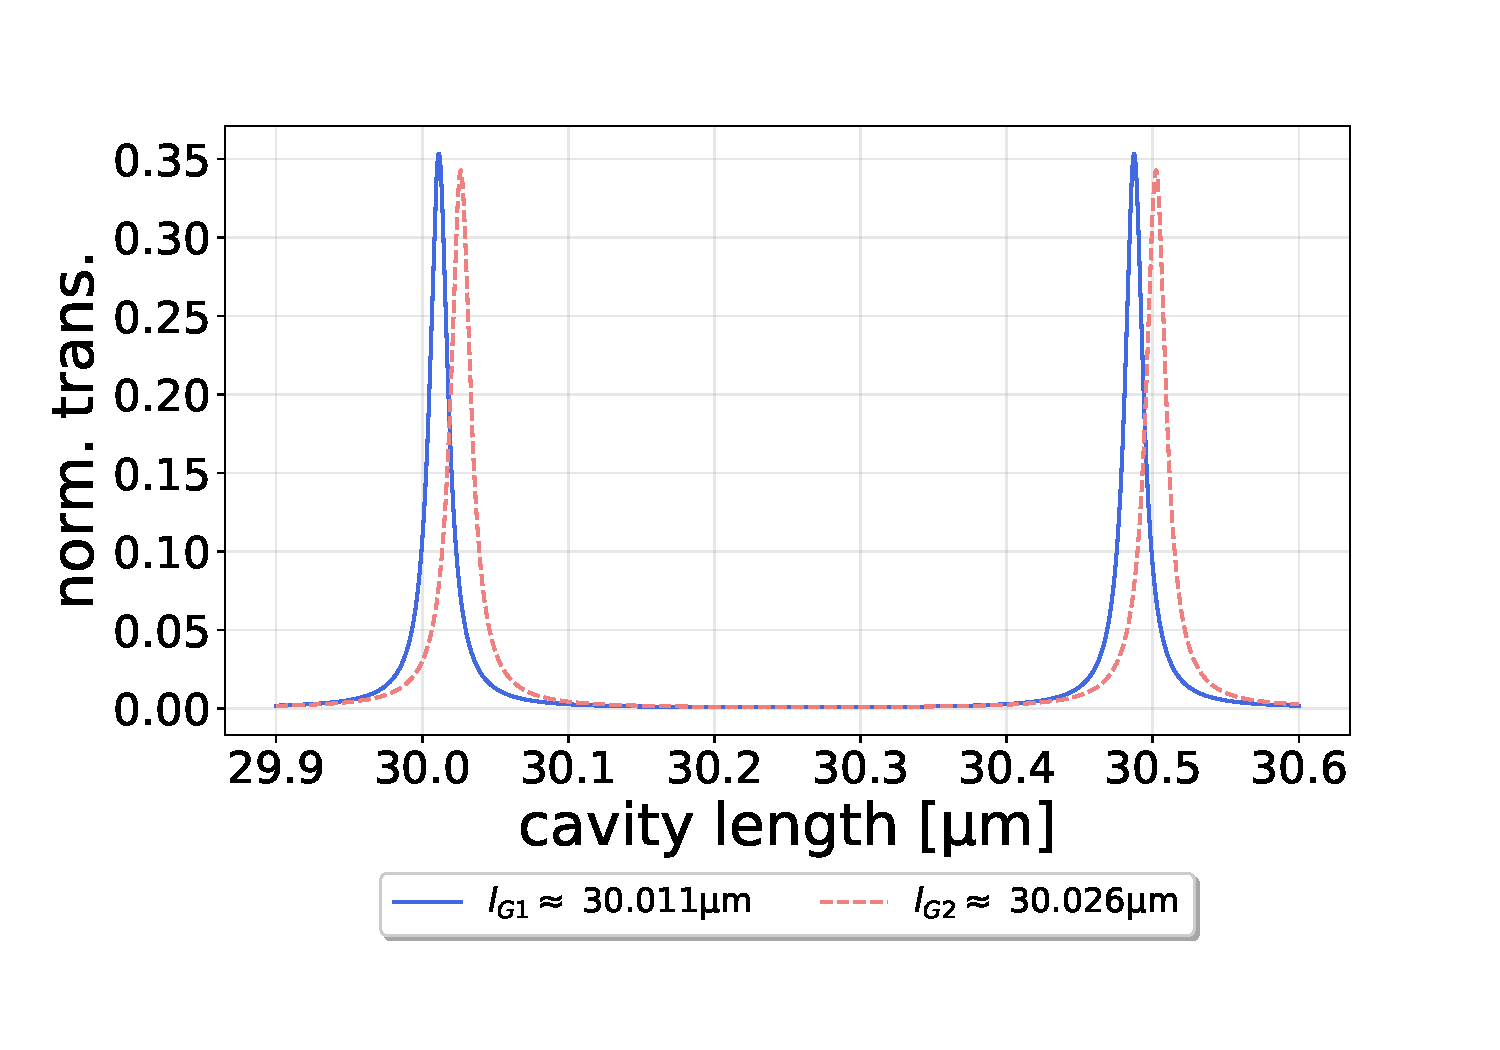
\includegraphics[width=0.7\textwidth]{figures/results/M3:M5_length_scan_sim_30um.pdf}
    \caption{}
    \label{fig:G1/G2_length_scan}
\end{figure}


\subsection{The single Fano cavity}\label{sec:the_single_fano_cavity_results}

We recall that the single fano cavity consists of a Fano mirror and a broadband mirror in a plane-plane configurations where each mirror is perpendicular to the optical axis. The single Fano cavity configuration is briefly outlined in section \ref{sec:cavity_measurements} and otherwise shown in \cite{Mitra}, it however resembles the double Fano cavity setup shown in figure \ref{fig:cavity_setup}, except only the bottom two xy-stages are used, and the top ones are therefore removed.   

The mirror used is a high relfective (HR) broadband mirror with a reflectivity of $99.7\%$, meaning that effectively all intrinsic cavity losses can be assumed to be associated with the Fano mirror. The Fano mirror used is G1 characterized in section \ref{sec:results_fano_mirror_characterization}. 

Figure \ref{fig:single_fano_fsr_scans} shows examples of off-resonance scans of the single Fano cavity, with corresponding fits to the Fabry-Perot transmission function, in order to determine the cavity length from the measured FSR. Figure \ref{fig:short_single_fano_FSR} shows the off-resonance spectrum for a cavity of length $l = 57.40 \pm 1.55 \mu m$, while figure \ref{fig:long_single_fano_FSR} shows the same for a cavity length of $l = 211.98 \pm 3.16 \mu m$. The errors are determined as the errors of the fit, found as the squareroot of the diagonal of the corresponding covariance matrices.

\begin{figure}[h!]
    \centering
    \begin{subfigure}[b]{0.49\textwidth}
        \centering
        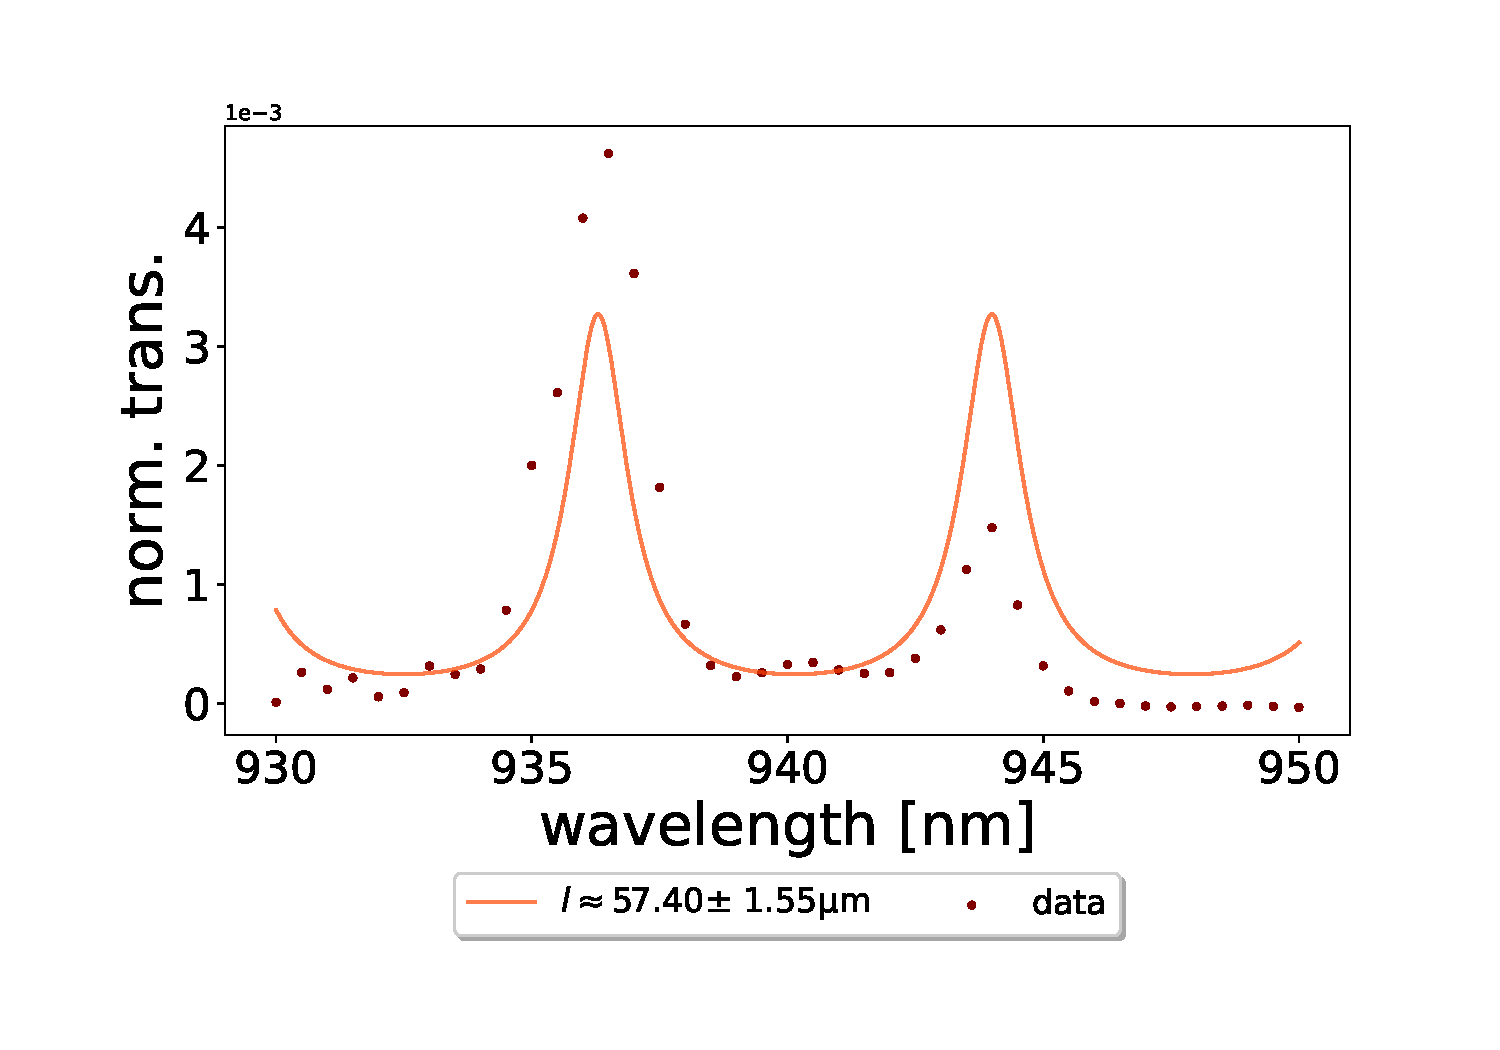
\includegraphics[width=\textwidth]{figures/results/single fano fits/60um_off_res_fabry_perot.pdf}
        \caption{}
        \label{fig:short_single_fano_FSR}
    \end{subfigure}
    \begin{subfigure}[b]{0.49\textwidth}
        \centering
        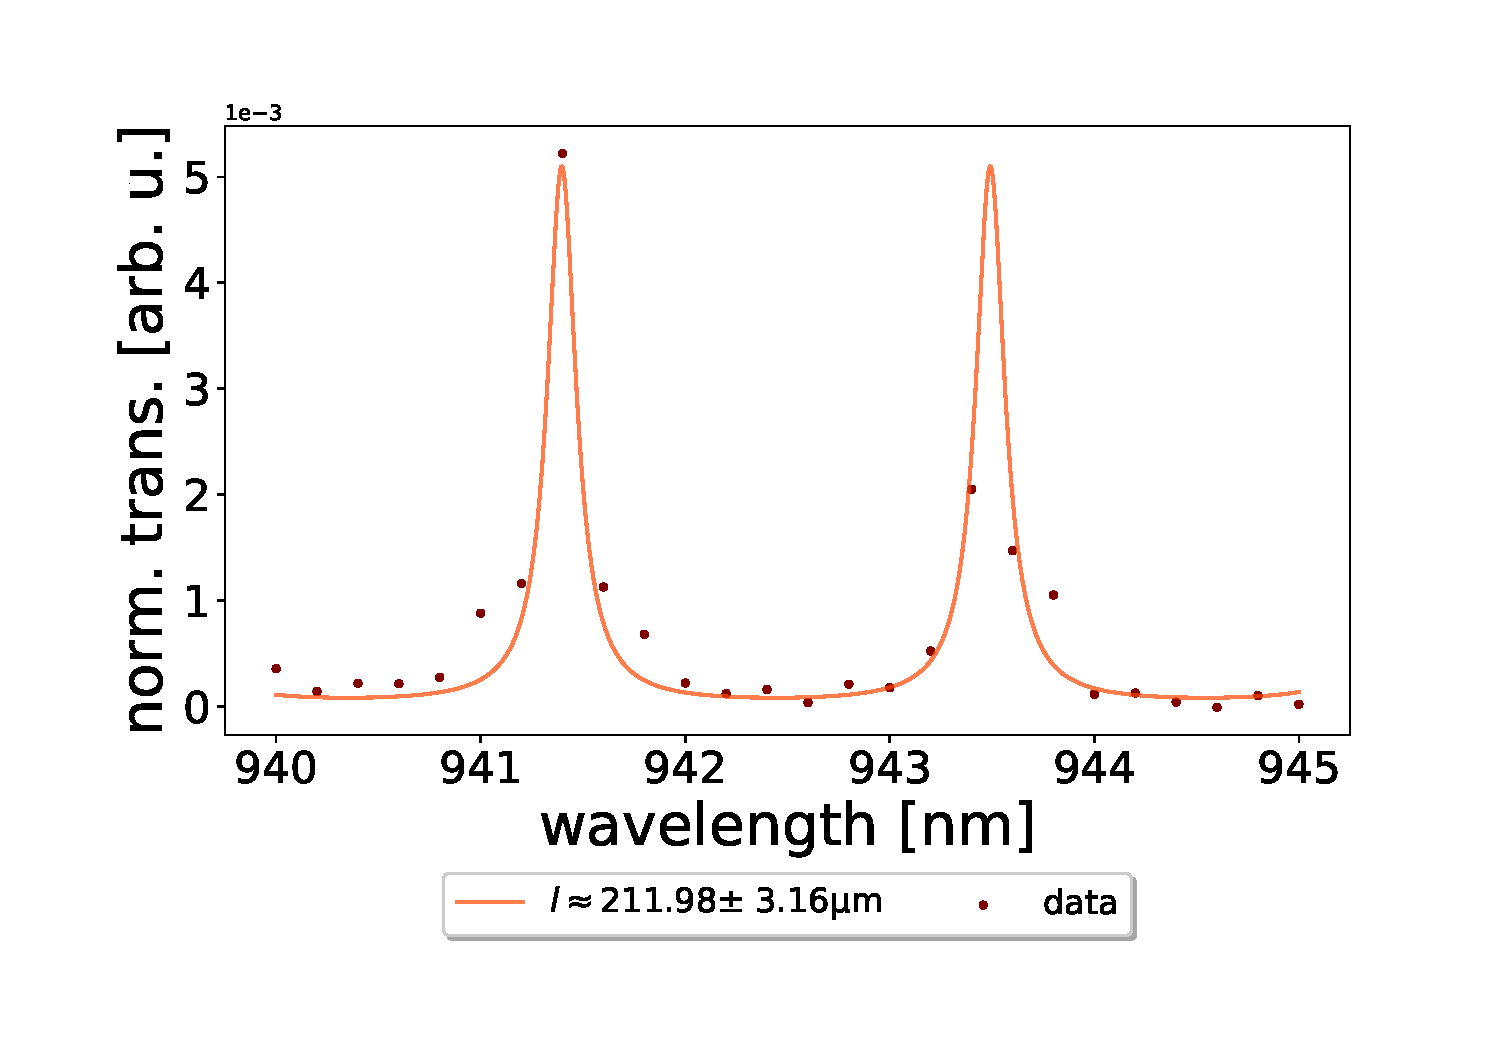
\includegraphics[width=\textwidth]{figures/results/single fano fits/220um_off_res_fabry_perot.pdf}
        \caption{}
        \label{fig:long_single_fano_FSR}
    \end{subfigure}
    \caption{}
    \label{fig:single_fano_fsr_scans}
\end{figure}

Figure \ref{fig:M5/G1_single_fano_trans_examples} shows examples of resonance transmission spectra of the single Fano cavity. The examples are taken for length corresponding to the ones found from the off-resonance spectra shown in figure \ref{fig:single_fano_fsr_scans} above. The figures are depicted with each their corresponding least squares fits to the generalized Fano model shown in eq. (\ref{eq:general_fano_model}) in order to determine the linewidth (HWHM) of the profile. The errors of the linewidths are found from the error of the fit and are mainly used to determine the quality of the measurement. 

\begin{figure}[h!]
    \centering
    \begin{subfigure}[b]{0.49\textwidth}
        \centering
        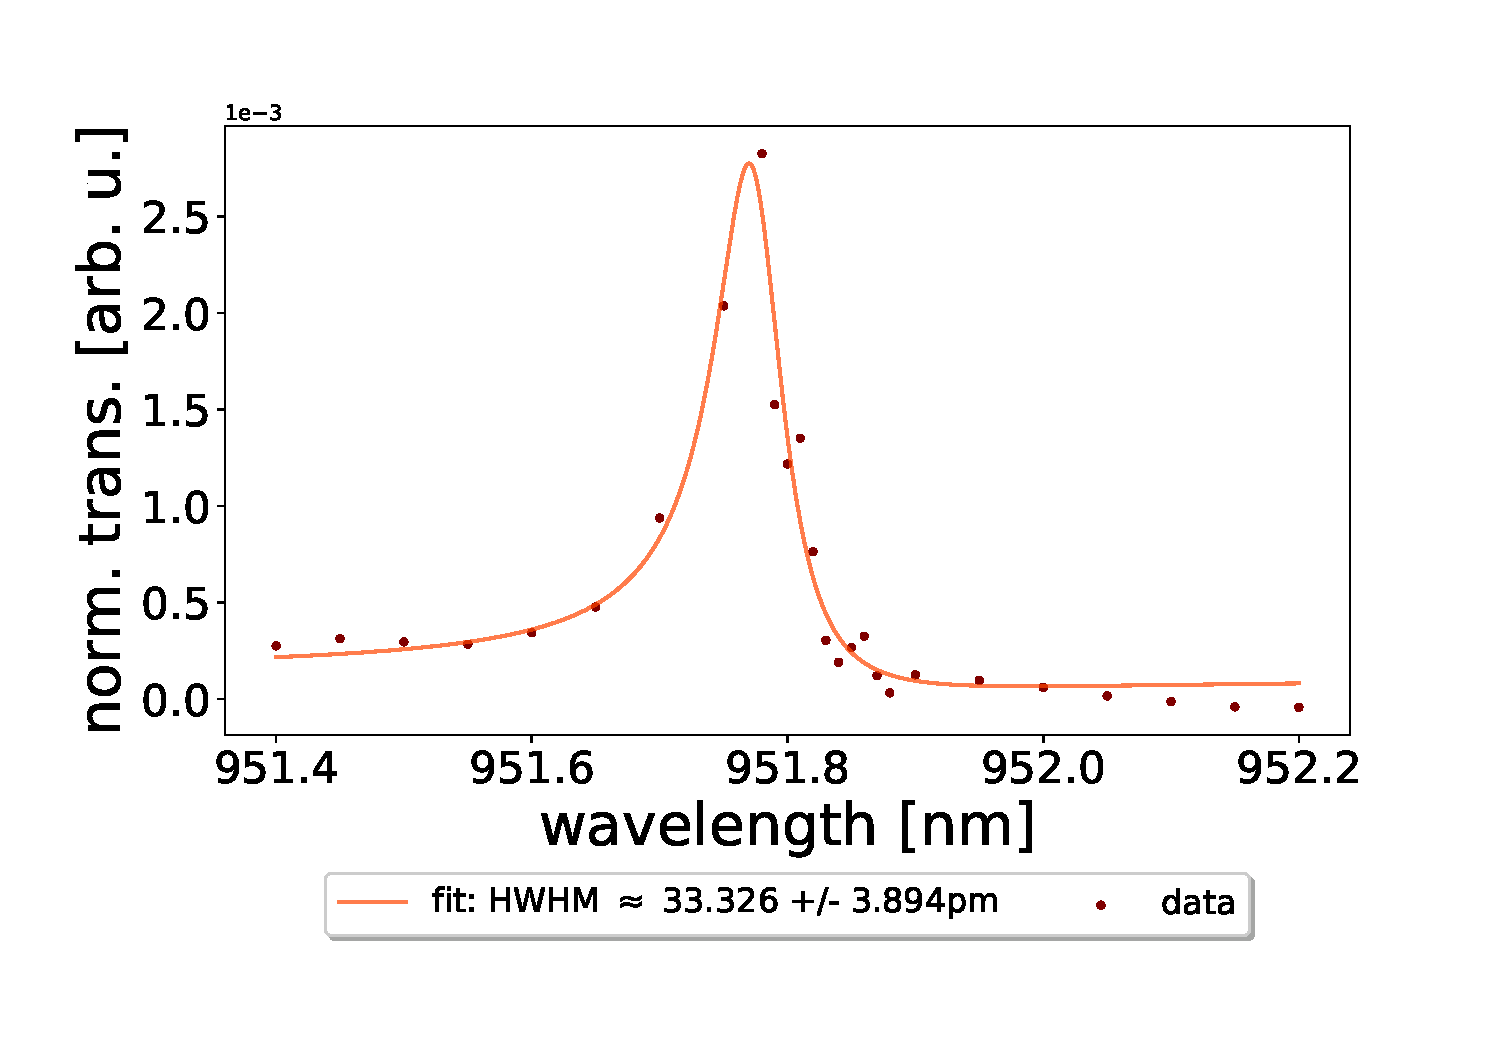
\includegraphics[width=\textwidth]{figures/results/single fano fits/60um_M5_fit_1.pdf}
        \caption{}
        \label{fig:short_single_fano_trans}
    \end{subfigure}
    \begin{subfigure}[b]{0.49\textwidth}
        \centering
        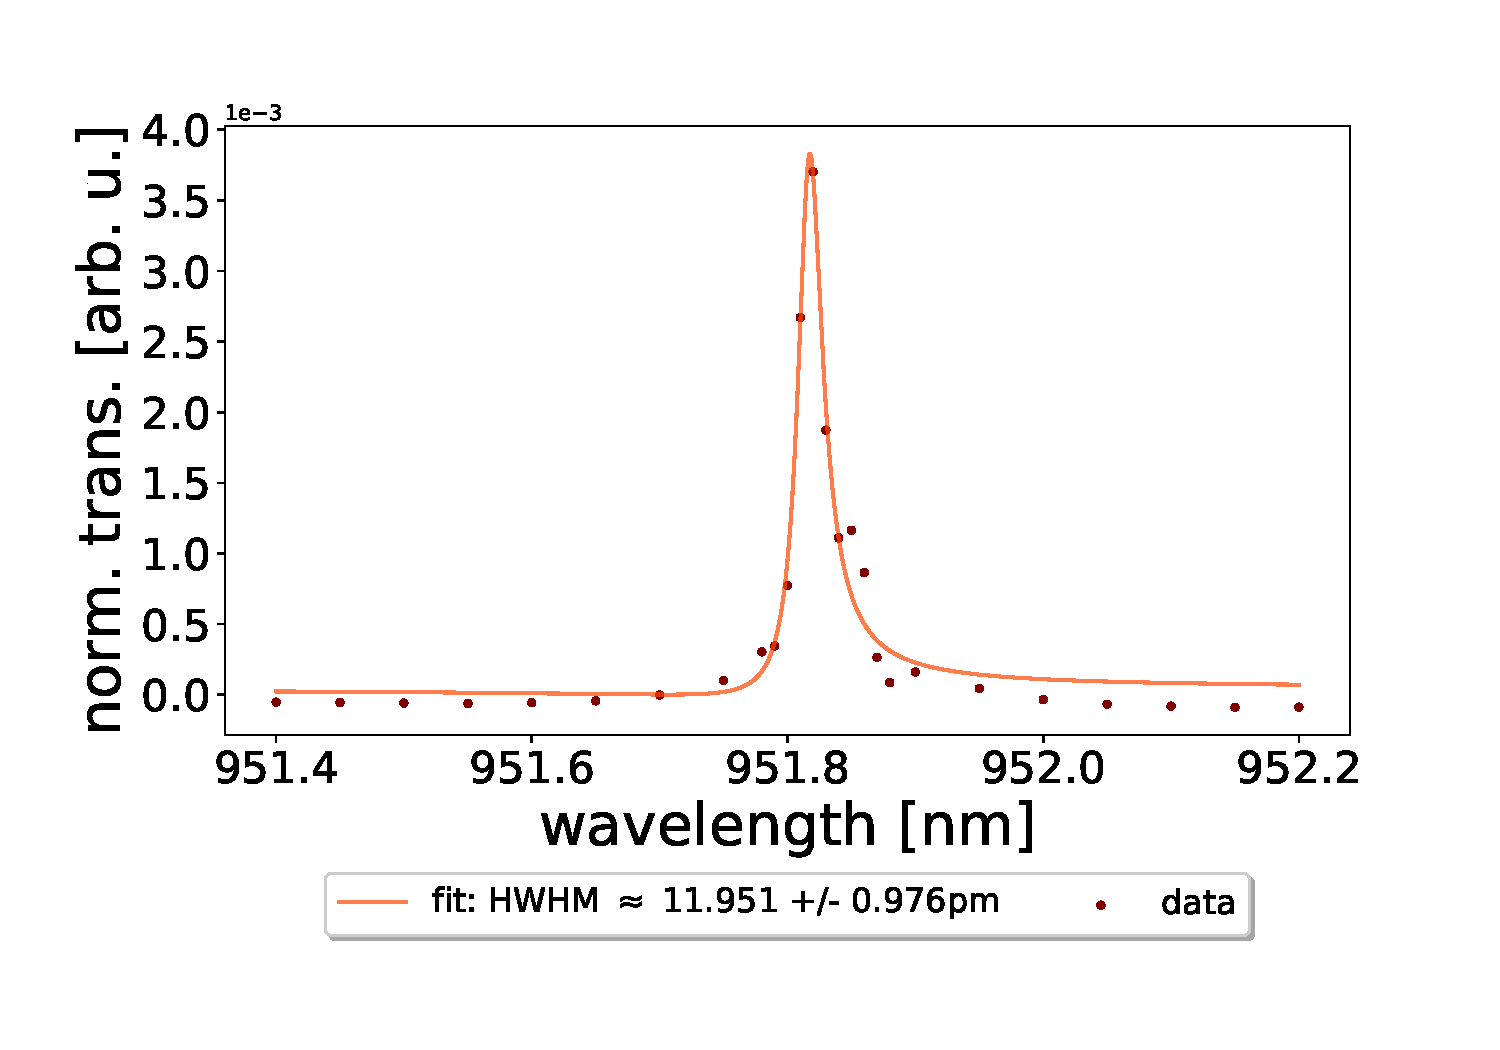
\includegraphics[width=\textwidth]{figures/results/single fano fits/220um_M5_fit_4.pdf}
        \caption{}
        \label{fig:long_single_fano_trans}
    \end{subfigure}
    \caption{}
    \label{fig:M5/G1_single_fano_trans_examples}
\end{figure}

At each cavity length, the resonance transmission profile was recorded a number of times and the average value was taken to be the found true value of the linewidth. Figure \ref{fig:HWHM_vs_time_single_fano_data} shows the result of a measurement series consisting of five cavity lengths approximately ranging from $20\mu m \leq l \leq 400 \mu m$, where the error of each measurement is given as the standard deviation of the values of all measurements recorded at each cavity length\cite{Hughes}. The error depicted in the x-direction is found from the error of the fit of the Fabry-Perot transmission function to the off-resonance spectra. The blue dashed line indicate the linewidth of a broadband cavity of similar losses according to eq. (\ref{eq:analytical_linewidth_broadband}) and the orange dashed line thus indicate the analytical linewidth of the single Fano cavity considered consisting of G1 and the HR broadband mirror estimated using eq. (\ref{eq:analytical_linewidth_single_fano}). The black points are linewidths found by fitting single Fano transmission profiles simulated using eq. (\ref{eq:single_fano_trans}) to the generalized Fano model in eq. (\ref{eq:general_fano_model}) for comparison. 

It is seen that the analytical model, the theoretically found linewidths and the measured linewidths coincide very well for the cavity lengths that are well-within the Fano regime and deviates slightly for longer lengths. This trend agrees nicely with what has previously been found for the single Fano cavity transmission\cite{Mitra} and is likely a consequence of the very narrow linewidths of the cavity in the standard regime, as this increases the sensitivity to any noise regarding the cavity length, e.g. mechanical vibrations in the setup.

\begin{figure}[h!]
    \centering
    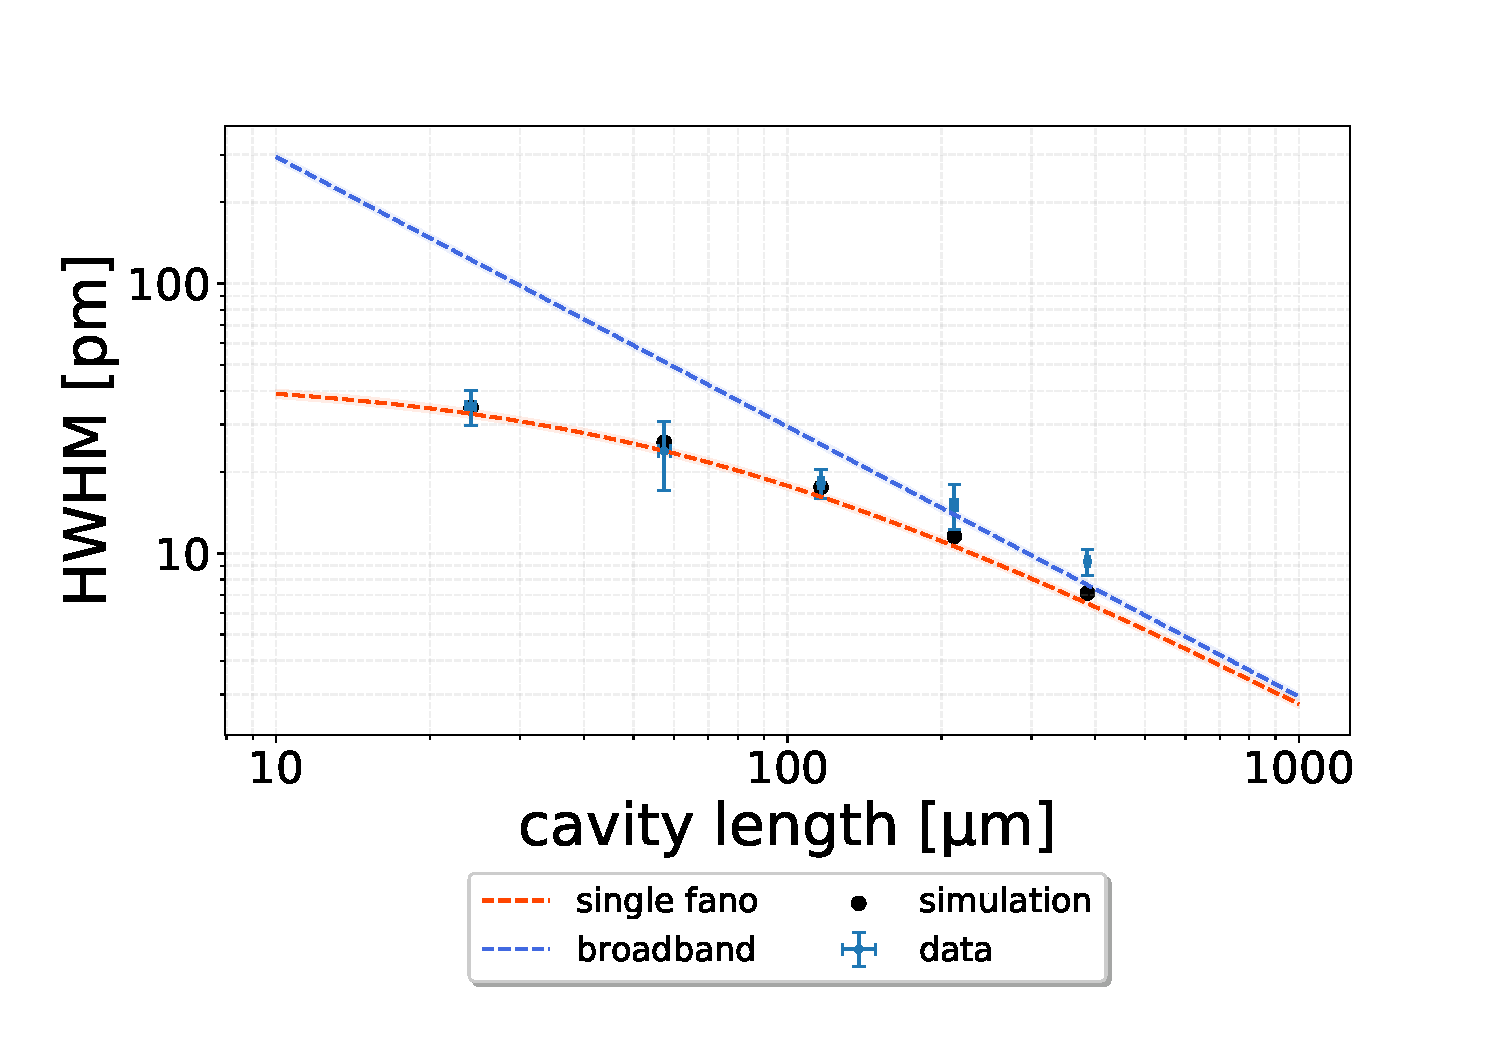
\includegraphics[width=0.7\textwidth]{figures/results/HWHM_vs_cavity_length_single_fano.pdf}
    \caption{}
    \label{fig:HWHM_vs_time_single_fano_data}
\end{figure}

\clearpage
\subsection{The double Fano cavity}\label{sec:the_double_fano_cavity_results}

In this section I will give an account of the results for the characterization of a double Fano cavity consisting of Fano mirrors G1 and G2. First we look at the simulated spectra of the double Fano transmission intensity profile as a function of the incident wavelength simulated with the parameters for G1 given in eq. (\ref{eq:G1_params}) and for G2 given in eq. (\ref{eq:G2_params}). Figures \ref{fig:G1_and_G2_full_range_spectra} and \ref{fig:G1_and_G2_short_range_spectra} shows the simulated spectra for cavity lengths according to $l=l_{G1}$, $l=l_{G2}$ and $l=(l_{G1}+l_{G2})/2$ together with the reflectivity spectra for G1 and G2 also shown in figure \ref{fig:G1_and_G2_spectral_comparison}. 

\begin{figure}[h!]
    \centering
    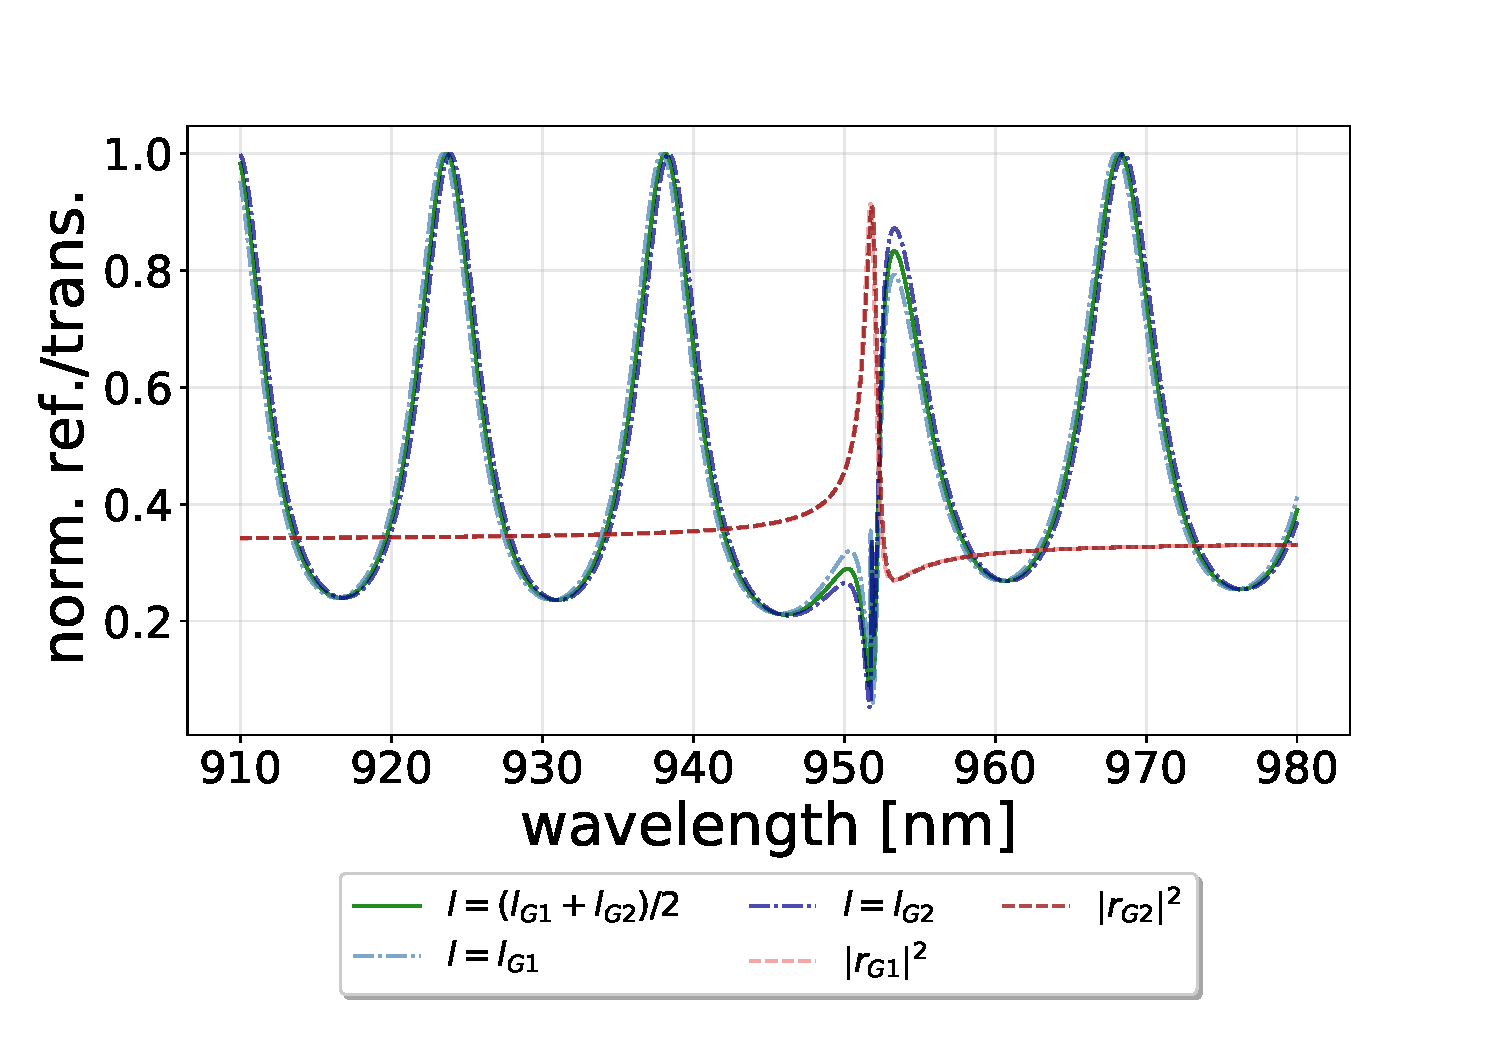
\includegraphics[width=0.7\textwidth]{figures/results/M3:M5/M3:M5_sim_spectra_long.pdf}
    \caption{}
    \label{fig:G1_and_G2_full_range_spectra}
\end{figure}

It is seen in figure \ref{fig:G1_and_G2_full_range_spectra} that the off-resonance level is expected to almost reach unity for a perfectly aligned cavity, for the given direct transmission amplitude coefficients $t_d$, $t_d^{\prime}$ and the same for the direct reflectivities $r_d$, $r_d^{\prime}$. This result for the simulated spectra is indicative of the validity of the assumption that these are at identical meaning that $t_{d,G1} \approx t_{d,G2}$ and $r_{d,G1} \approx r_{d,G2}$. Furthermore, the background perfectly resembles a low finesse Fabry-Perot cavity, as is expected from the theory. 

Figure \ref{fig:G1_and_G2_short_range_spectra} shows the transmission spectra of the doubel Fano cavity zoomed on the resonance wavelengths considered according to the depicted cavity lengths. Here it is seen how the transmission peak at resonance is expected to shift with the cavity length, and that the estimated detuning $\Delta$ of the two Fano mirrors seems to be sufficiently small in order to realize the double Fano resonance profile. Lastly, it is seen what to expect in terms of the peak height of the resonance profile as this is an important merit when practically estimating the losses, and by extension the alignment, of the cavity in the lab. 

\begin{figure}[h!]
    \centering
    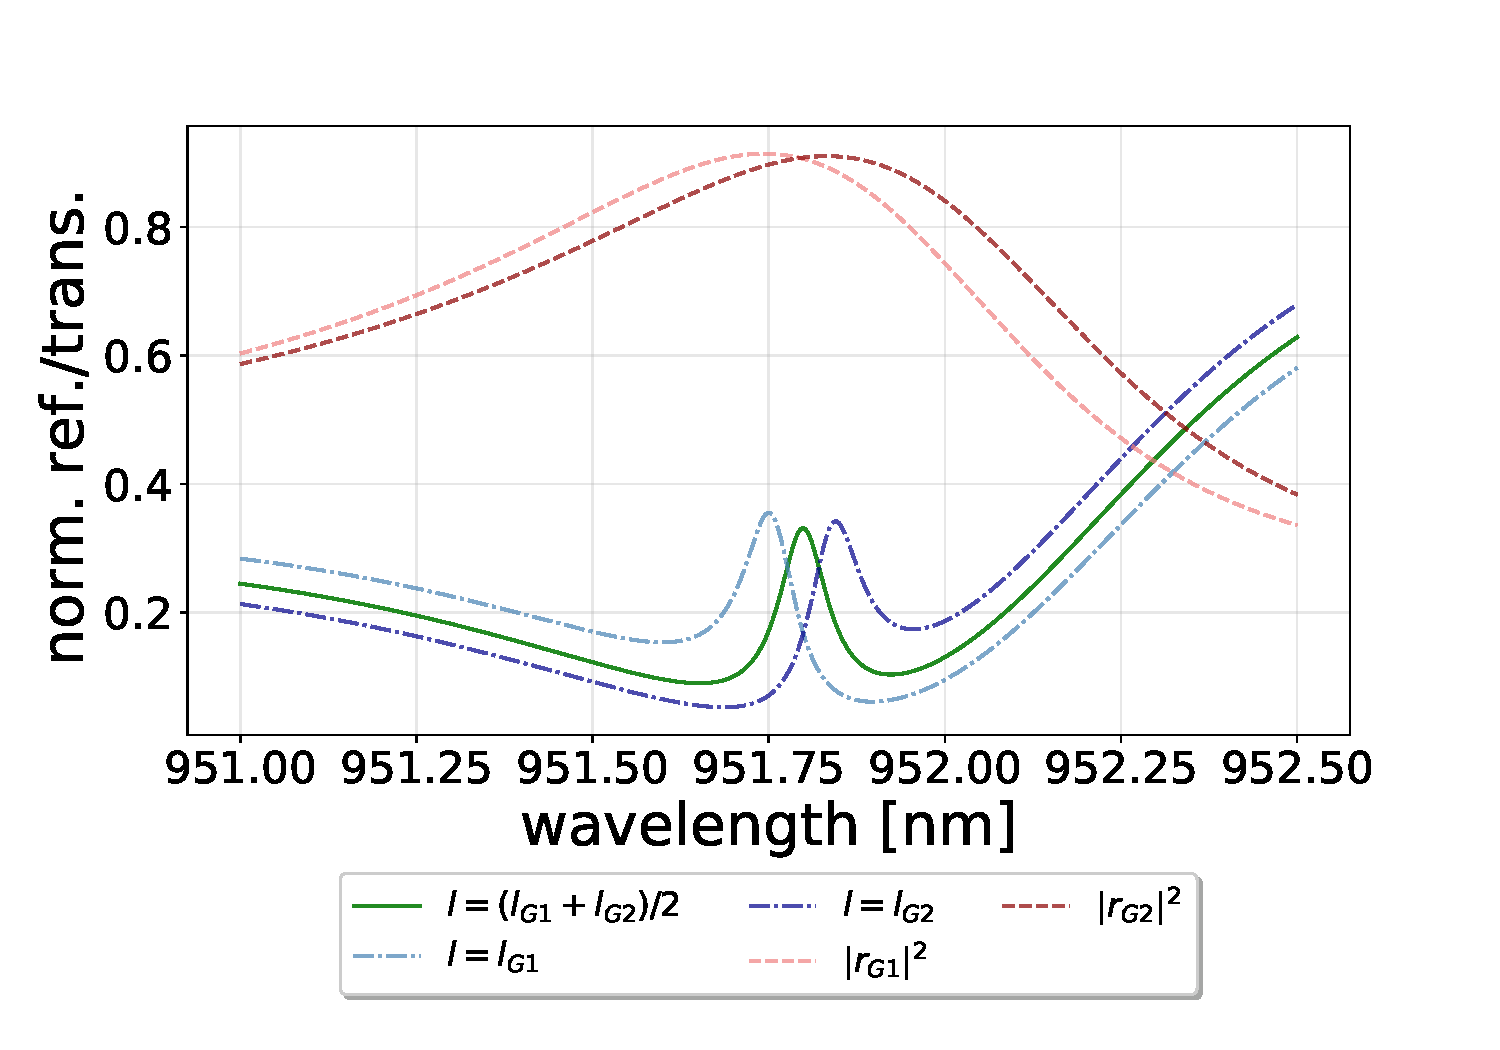
\includegraphics[width=0.7\textwidth]{figures/results/M3:M5/M3:M5_sim_spectra_short.pdf}
    \caption{}
    \label{fig:G1_and_G2_short_range_spectra}
\end{figure}

I simulate the transmission profile for different cavity length in order to determine the optimal one. Figure \ref{fig:G1_G2_cmap} shows a colormap of the resonance profile as a function of wavelength and cavity lengths ranging $l_{G1} \leq l \leq l_{G2}$. The peak height is indicated by the brightness of the colormap, such that the resonance wavelength and cavity length is indicated by the "line" showing the resonance peak moving in terms of both parameters. 

\begin{figure}[h!]
    \centering
    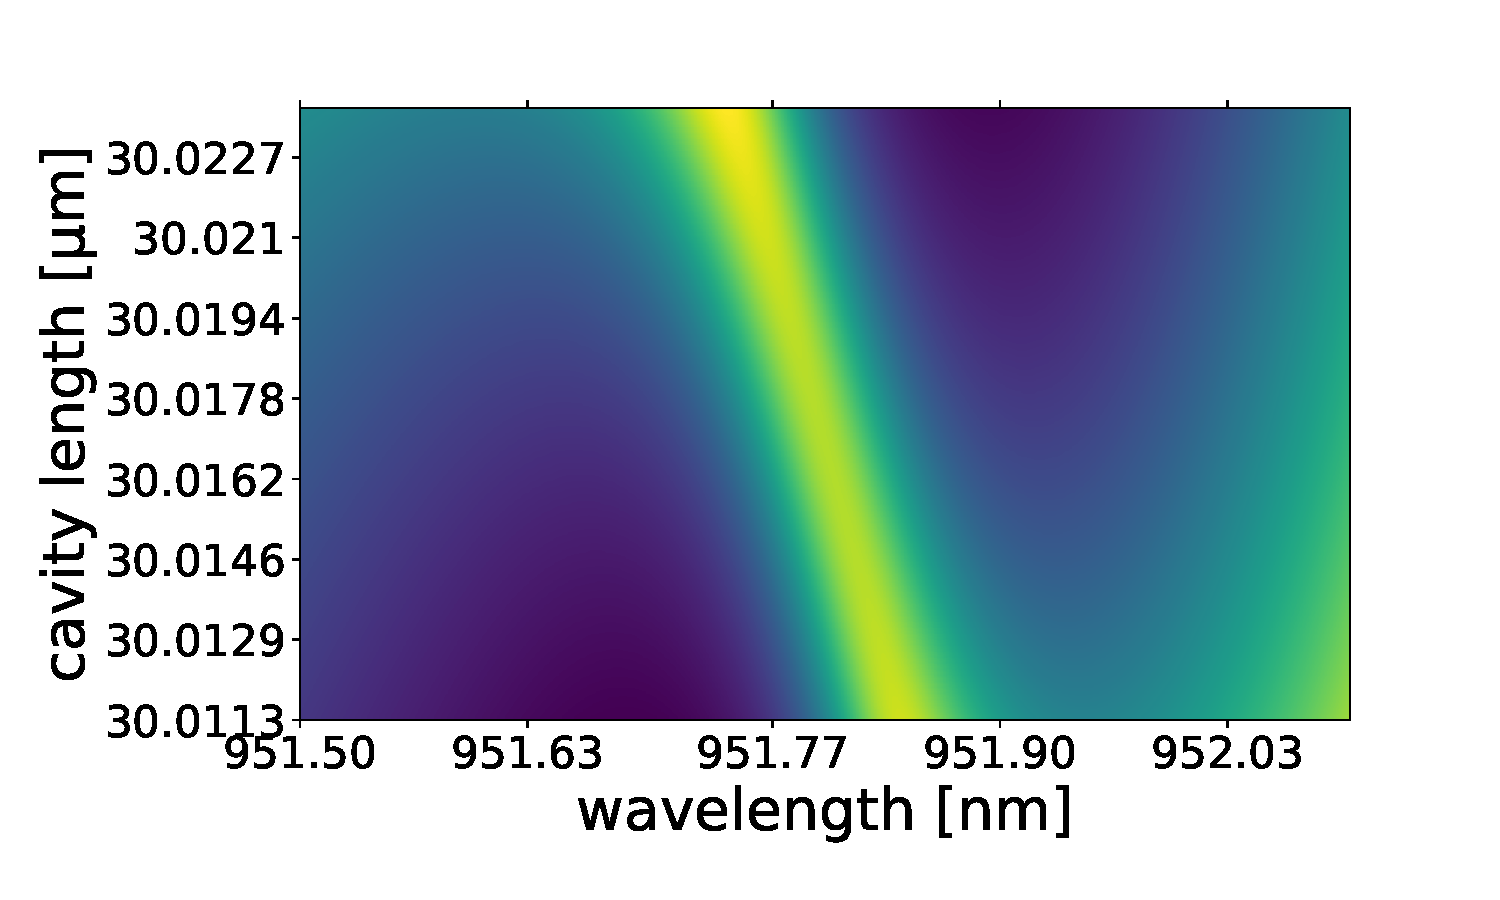
\includegraphics[width=0.7\textwidth]{figures/results/M3:M5/G1:G2_cmap.pdf}
    \caption{}
    \label{fig:G1_G2_cmap}
\end{figure}

The colormap provides a qualitative and intuitive image of the behaviour of the double Fano transmission profile, but the optimal cavity length in order to optimize with respect to the linewidth is nearly imposible to determine. Figure \ref{fig:G1/G2_lw_vs_cavity_length} instead shows the linewidth of intracavity spectra as a function of the cavity length and shows that the optimal cavity length is approximately given as $l \approx (l_{G1} + l_{G2})/2$. In reality, the assymetric structure of the Fano mirror spectra results in an exact answer to the optimal cavity that is more complicated, and likely impossible to realize in the lab. For this reason the approximate interpretation of the cavity length analysis is sufficient for practical purposes.

\begin{figure}[h!]
    \centering
    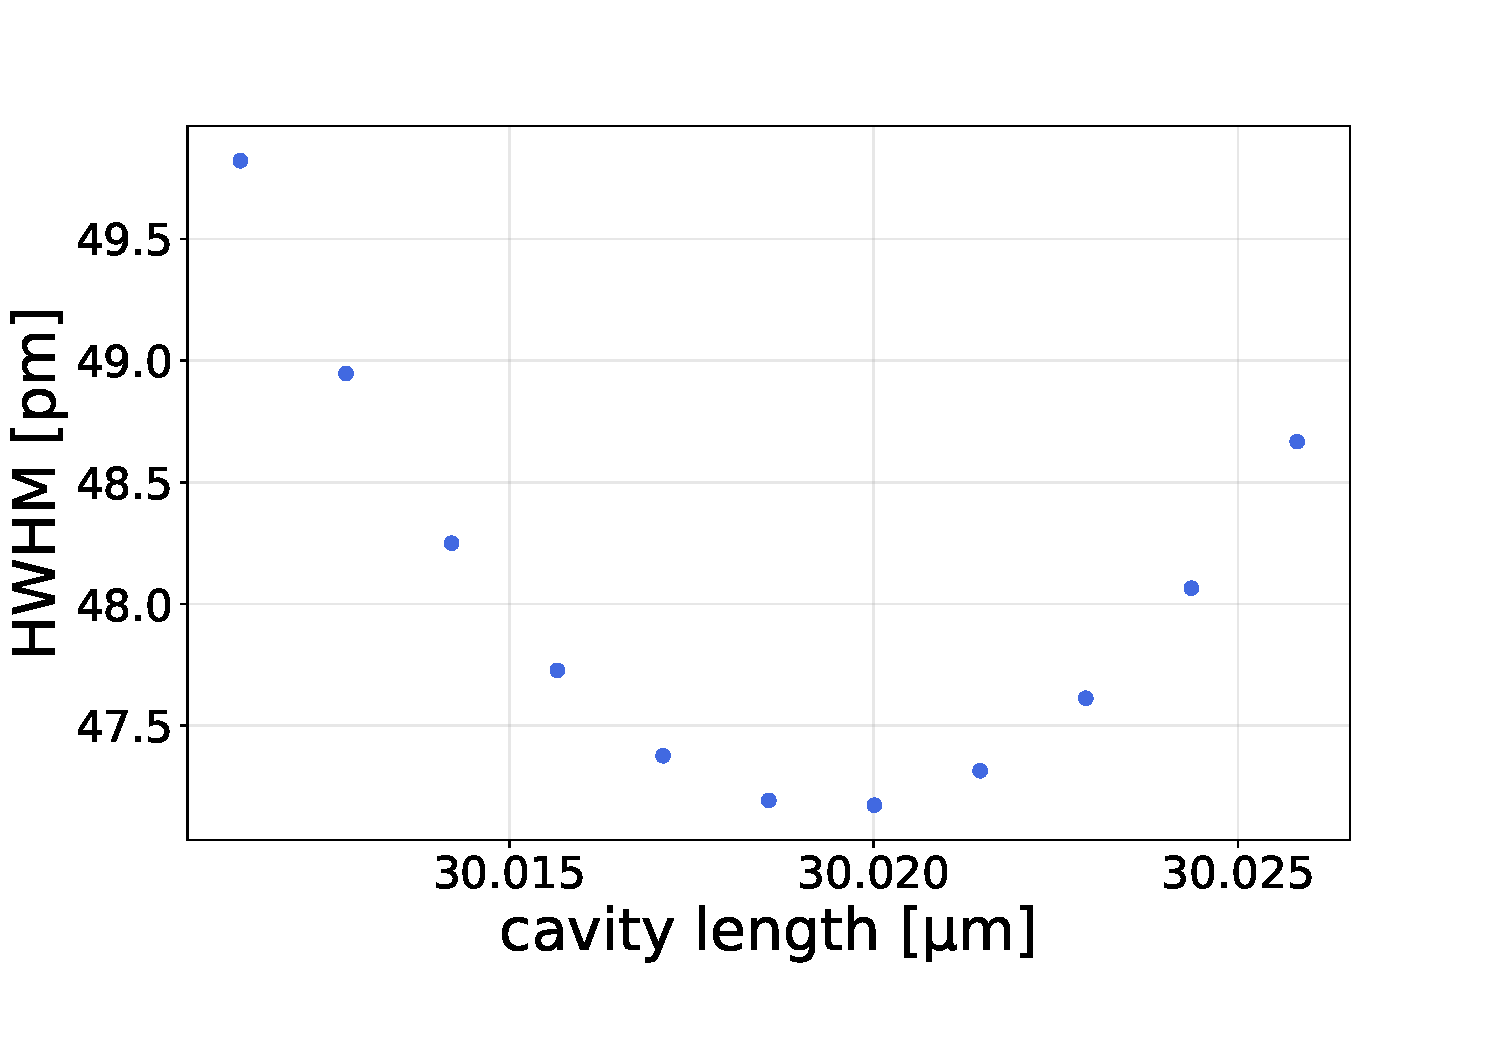
\includegraphics[width=0.7\textwidth]{figures/results/M3:M5/M3:M5_lw_vs_length.pdf}
    \caption{}
    \label{fig:G1/G2_lw_vs_cavity_length}
\end{figure}

\subsubsection{Realizing the double fano model}\label{sec:realizing_the_double_fano_model}

In order to realize the double Fano model in a satisfying way the whole spectrum is examined as the off-resonance profile resembling a low-finesse Fabry-Perot transmission spectrum, with near-unity transmission levels at each "Fabry-Perot" peak, is considered a defining feature of the double Fano cavity. In this section I will present three spectra obtained experimentally and compared with their corresponding simulated spectra for lengths $l=l_{G1}$, $l=l_{G2}$ and $l=(l_{G1} + l_{G2})/2$. Furthermore, I present the same spectra fitted to the double Fano cavity transmission model with fitting parameters given as the two sets of Fano mirror parameters, the cavity length and the resonant loss term $L$. The Fano mirror parameters found by the fitting function will thus be those that produce the reflection and transmission amplitude coefficients that best fit the data. 

\begin{figure}[h!]
    \centering
    \begin{subfigure}[b]{0.49\textwidth}
        \centering
        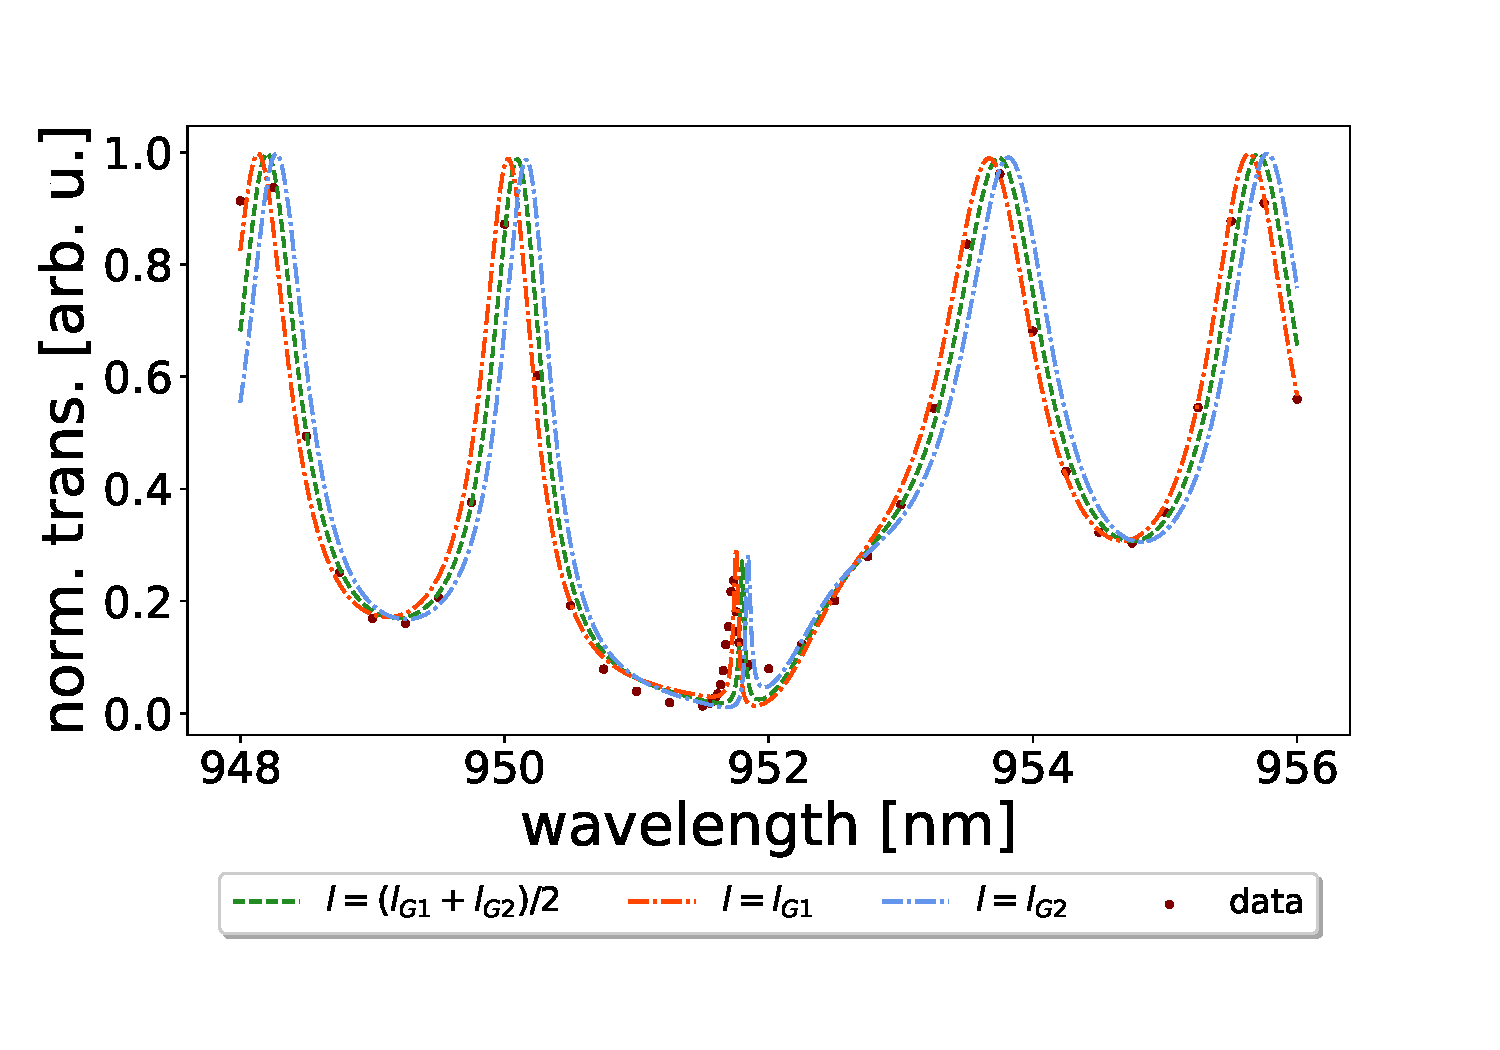
\includegraphics[width=\textwidth]{figures/results/238um_long_scan_sim_comparison.pdf}
        \caption{}
        \label{fig:238um_long_scan_sim_comparison}
    \end{subfigure}
    \begin{subfigure}[b]{0.49\textwidth}
        \centering
        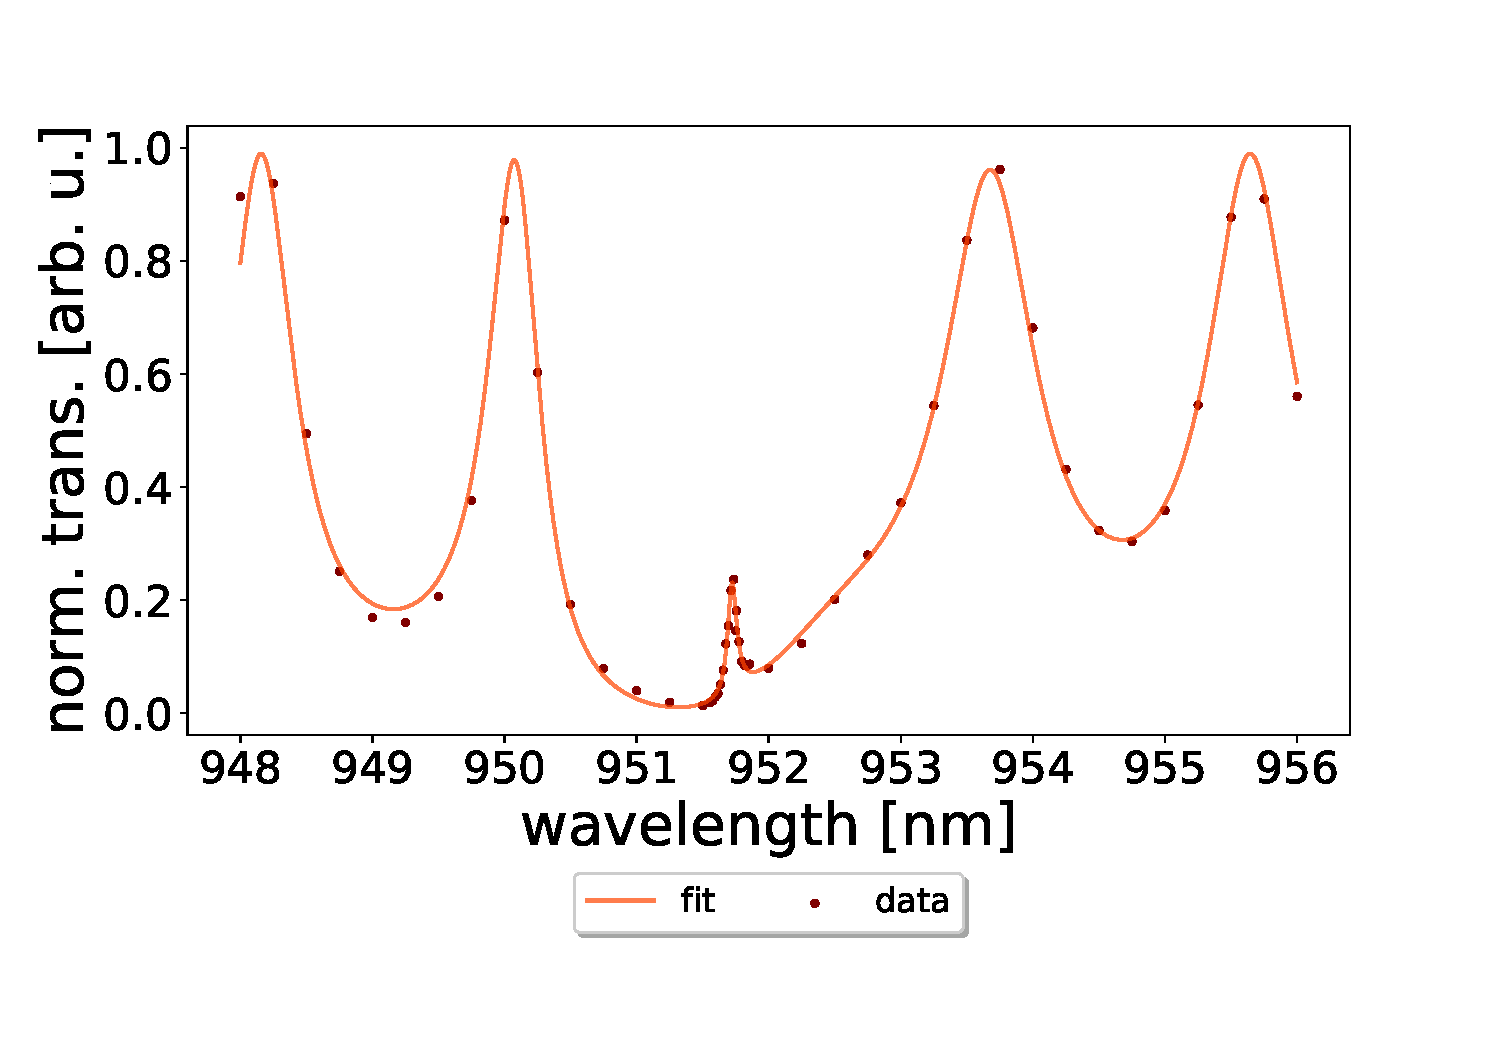
\includegraphics[width=\textwidth]{figures/results/238um_long_scan_fit.pdf}
        \caption{}
        \label{fig:238um_long_scan_fit}
    \end{subfigure}
    \caption{$l_{G1} = 239.3975 \mu m$, $l_{G2} = 239.4317 \mu m$, $(l_{G1} + l_{G2})/2 = 239.4146 \mu m$}
    \label{fig:238um_cavity_fit_and_sim}
\end{figure}

Figure \ref{fig:238um_long_scan_sim_comparison} show the comparison of data and simulation for a cavity of lengths given as $l_{G1} = 239.3975 \mu m$, $l_{G2} = 239.4317 \mu m$, $(l_{G1} + l_{G2})/2 = 239.4146 \mu m$. Figure \ref{fig:238um_long_scan_fit} shows a least squares fit of the data to the double Fano transmission function with fitting parameters related to each Fano mirror, and the cavity as follows.

Fitting parameters related to Fano mirror G1:
\begin{equation}
    \begin{split}
        \lambda_0 = 9&51.330 \pm 0.072 \text{nm}, \:\: \lambda_1 = 951.328 \pm 0.110 \text{nm}, \:\: t_d = 0.827 \pm 0.016, \:\: \\&\gamma_{\lambda} = 0.641 \pm 0.131 \text{nm}, \:\: \beta = 1.819 \cdot 10^{-6} \pm 9.314 \cdot 10^{-7} \text{m}^{-1}.
    \end{split}
\end{equation}

Fitting parameters related to Fano mirror G2:
\begin{equation}
    \begin{split}
        \lambda_0 = 9&51.728 \pm 0.027 \text{nm}, \:\: \lambda_1 = 951.943 \pm 0.0428 \text{nm}, \:\: t_d = 0.823 \pm 0.015, \:\: \\&\gamma_{\lambda} = 0.535 \pm 0.056 \text{nm}, \:\: \beta = 7.788 \cdot 10^{-7} \pm 1.480 \cdot 10^{-7} \text{m}^{-1}.
    \end{split}
\end{equation}

Fitting parameters related to the cavity configuration:
\begin{equation}
    l = 238.924 \pm 0.002 \mu m, \:\: L = 0.039 \pm 0.099.
\end{equation}

\begin{figure}[h!]
    \centering
    \begin{subfigure}[b]{0.49\textwidth}
        \centering
        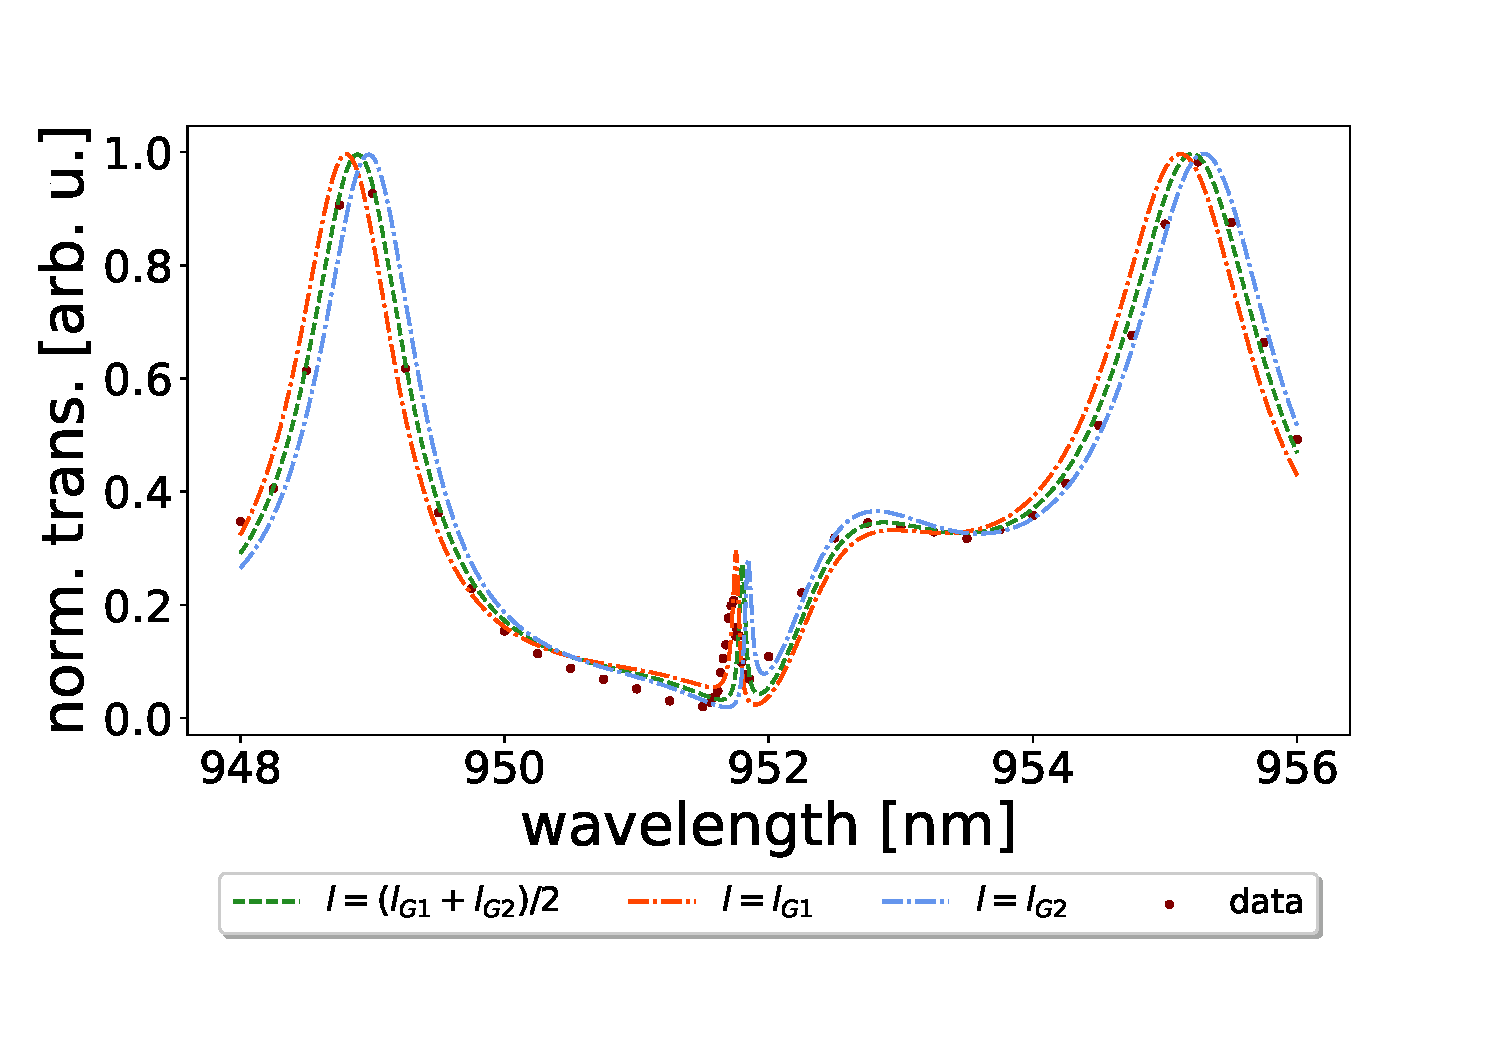
\includegraphics[width=\textwidth]{figures/results/129um_long_scan_sim_comparison.pdf}
        \caption{}
        \label{fig:129um_long_scan_sim_comparison}
    \end{subfigure}
    \begin{subfigure}[b]{0.49\textwidth}
        \centering
        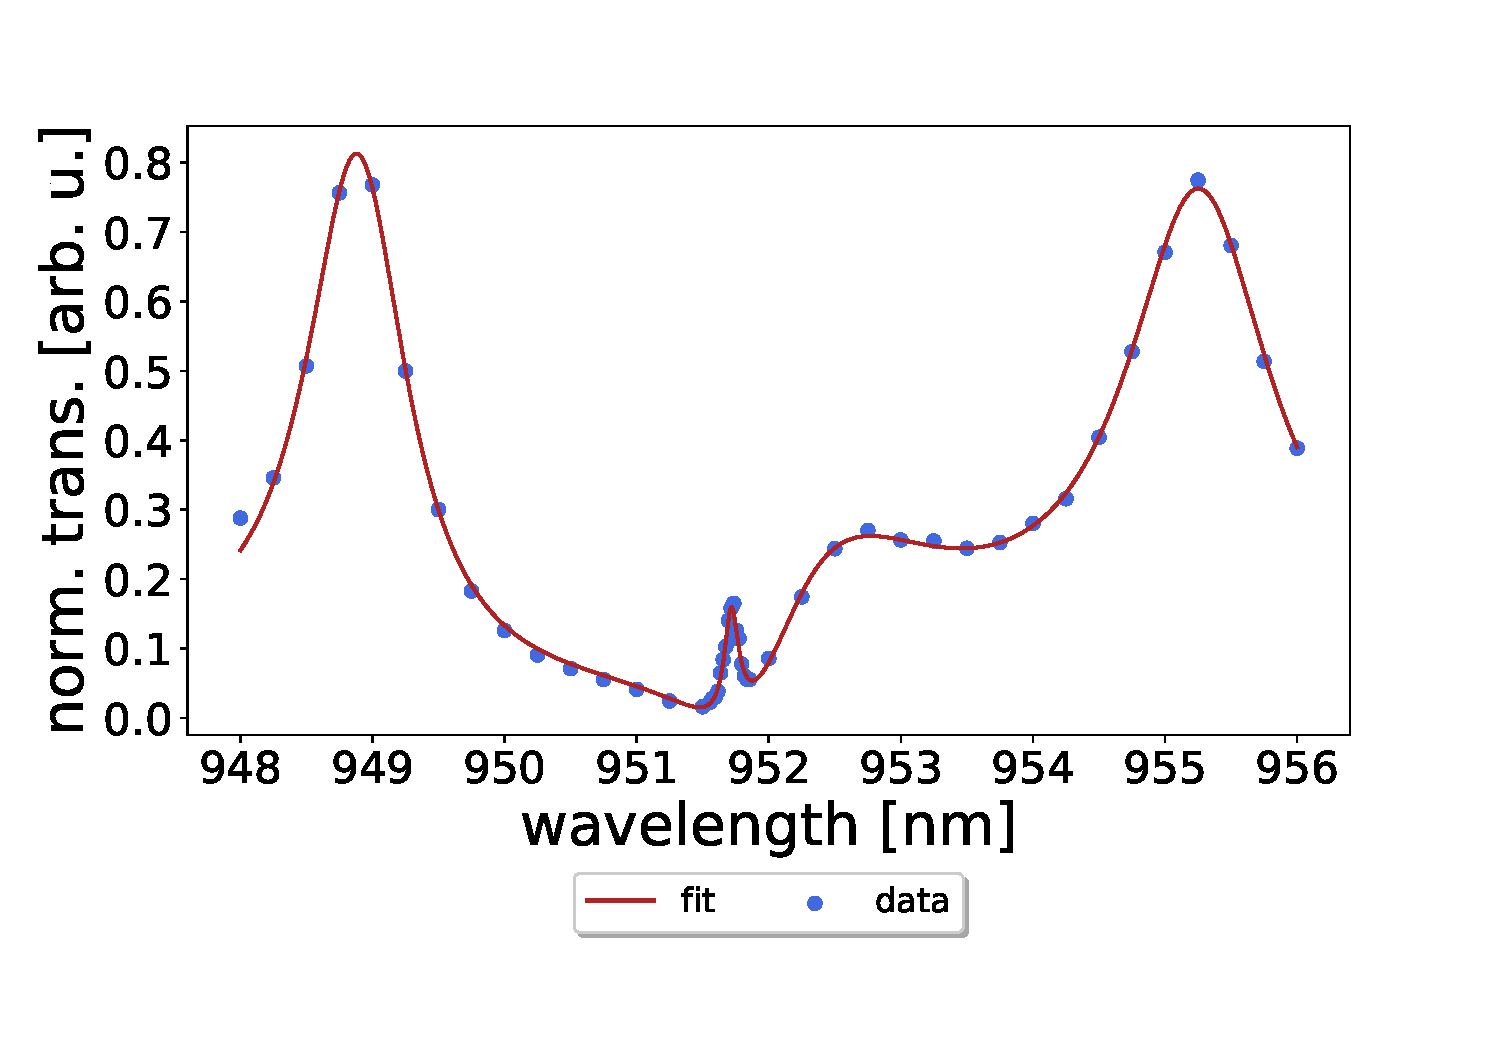
\includegraphics[width=\textwidth]{figures/results/129um_long_scan_fit.pdf}
        \caption{}
        \label{fig:129um_long_scan_fit}
    \end{subfigure}
    \caption{$l_{G1} = 140.4152 \mu m$, $l_{G2} = 140.4401 \mu m$, $(l_{G1} + l_{G2})/2 = 140.4277 \mu m$}
    \label{fig:129um_cavity_fit_and_sim}
\end{figure}

Figure \ref{fig:129um_long_scan_sim_comparison} show the comparison of data and simulation for a cavity of lengths given as $l_{G1} = 140.4152 \mu m$, $l_{G2} = 140.4401 \mu m$, $(l_{G1} + l_{G2})/2 = 140.4277 \mu m$. Figure \ref{fig:129um_long_scan_fit} shows a least squares fit of the data to the double Fano transmission function with fitting parameters related to each Fano mirror, and the cavity as follows.

Fitting parameters related to Fano mirror G1:
\begin{equation}
    \begin{split}
        \lambda_0 = 9&51.485 \pm 0.035 \text{nm}, \:\: \lambda_1 = 951.709 \pm 0.036 \text{nm}, \:\: t_d = 0.823 \pm 0.009, \:\: \\&\gamma_{\lambda} = 0.549 \pm 0.039 \text{nm}, \:\: \beta = 1.187 \cdot 10^{-6} \pm 2.810 \cdot 10^{-7} \text{m}^{-1}.
    \end{split}
\end{equation}

Fitting parameters related to Fano mirror G2:
\begin{equation}
    \begin{split}
        \lambda_0 = 9&51.799 \pm 0.020 \text{nm}, \:\: \lambda_1 = 951.852 \pm 0.0433 \text{nm}, \:\: t_d = 0.816 \pm 0.010, \:\: \\&\gamma_{\lambda} = 0.548 \pm 0.043 \text{nm}, \:\: \beta = 8.335 \cdot 10^{-7} \pm 1.105 \cdot 10^{-7} \text{m}^{-1}.
    \end{split}
\end{equation}

Fitting parameters related to the cavity configuration:
\begin{equation}
    l = 139.003 \pm 0.001 \mu m, \:\: L = 0.143 \pm 0.037.
\end{equation}

\begin{figure}[h!]
    \centering
    \begin{subfigure}[b]{0.49\textwidth}
        \centering
        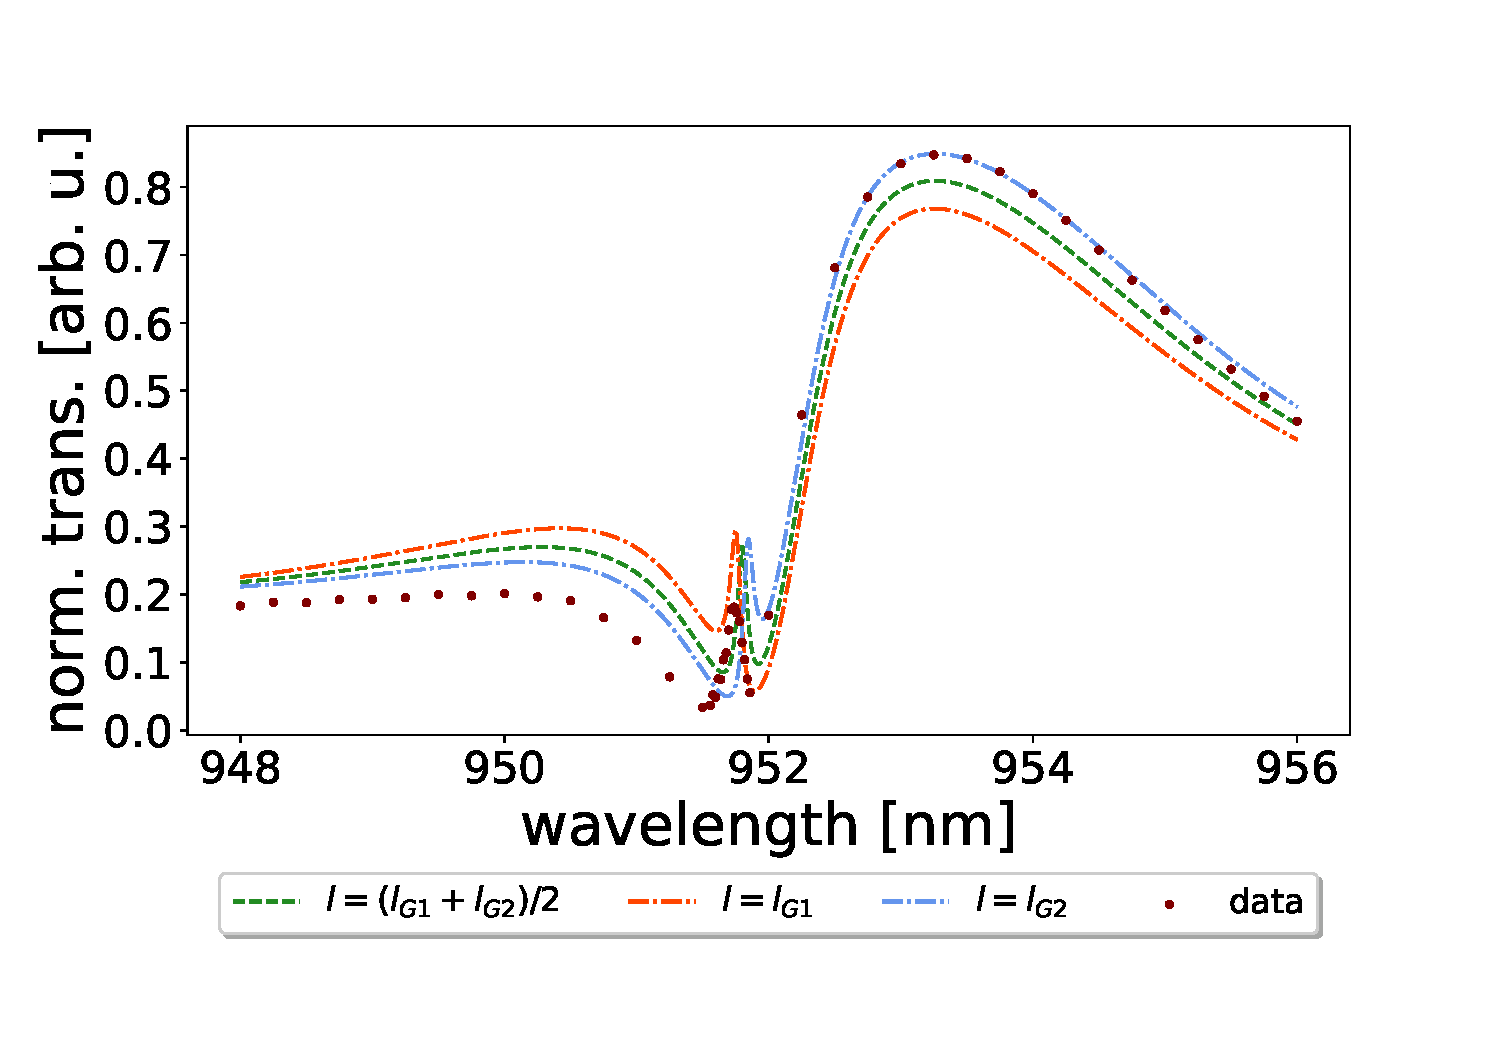
\includegraphics[width=\textwidth]{figures/results/34um_long_scan_sim_comparison.pdf}
        \caption{}
        \label{fig:34um_long_scan_sim_comparison}
    \end{subfigure}
    \begin{subfigure}[b]{0.49\textwidth}
        \centering
        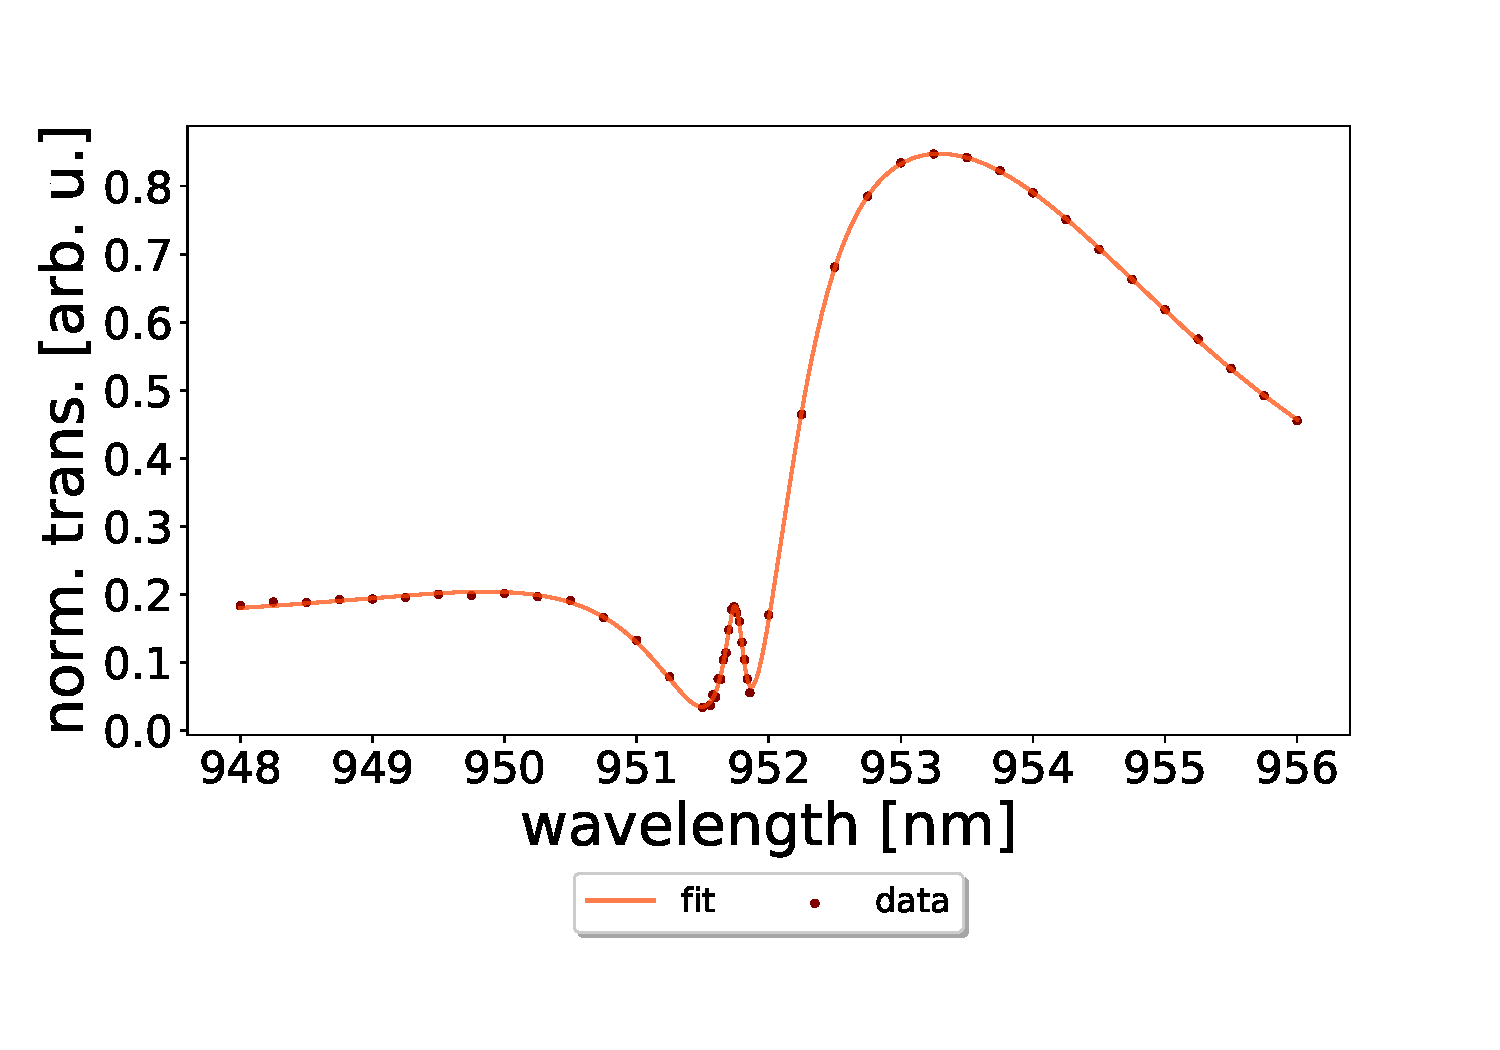
\includegraphics[width=\textwidth]{figures/results/34um_long_scan_fit.pdf}
        \caption{}
        \label{fig:34um_long_scan_fit}
    \end{subfigure}
    \caption{$l_{G1} = 33.3424 \mu m$, $l_{G2} = 33.3573 \mu m$, $(l_{G1} + l_{G2})/2 = 33.3499 \mu m$}
    \label{fig:34um_cavity_fit_and_sim}
\end{figure}

Figure \ref{fig:34um_long_scan_sim_comparison} show the comparison of data and simulation for a cavity of lengths given as $l_{G1} = 33.3424 \mu m$, $l_{G2} = 33.3573 \mu m$, $(l_{G1} + l_{G2})/2 = 33.3499 \mu m$. Figure \ref{fig:34um_long_scan_fit} shows a least squares fit of the data to the double Fano transmission function with fitting parameters related to each Fano mirror, and the cavity as follows.

Fano mirror \emph{G1} fitting parameters:
\begin{equation}
    \begin{split}
        \lambda_0 = 9&51.532 \pm 0.008 \text{nm}, \:\: \lambda_1 = 951.689 \pm 0.074 \text{nm}, \:\: t_d = 0.817 \pm 0.027, \:\: \\&\gamma_{\lambda} = 0.421 \pm 0.134 \text{nm}, \:\: \beta = 1.047 \cdot 10^{-6} \pm 4.947 \cdot 10^{-8} \text{m}^{-1}.
    \end{split}
\end{equation}

Fano mirror \emph{G2} fitting parameters:
\begin{equation}
    \begin{split}
        \lambda_0 = 9&51.853 \pm 0.004 \text{nm}, \:\: \lambda_1 = 951.919 \pm 0.017 \text{nm}, \:\: t_d = 0.754 \pm 0.033, \:\: \\&\gamma_{\lambda} = 0.563 \pm 0.079 \text{nm}, \:\: \beta = 5.245 \cdot 10^{-7} \pm 2.823 \cdot 10^{-8} \text{m}^{-1}.
    \end{split}
\end{equation}

Cavity parameters:
\begin{equation}
    l = 30.984 \pm 0.006 \mu m, \:\: L = 0.017 \pm 0.184.
\end{equation}

\subsubsection*{Comparison with simulations}

In all cases shown above the data and corresponding simulation shows remarkable overlap and agreement, as most data points are placed within, or very close to, the area enclosed by the simulations for the three considered cavity lengths. While this is only a qualitative measure, it indicates a high level of predictive strength of the model outlined in section \ref{sec:fano_mirror} and eq. (\ref{eq:double_fano_transmission}) and likewise for the experimental method used shown in section \ref{sec:cavity_measurements}.

\subsubsection*{Fits to the double Fano model}

All optical parameters for G1 and G2 found as fitting parameters of the double Fano model are approximately in agreement with the ones found for G1 and G2 in section \ref{sec:results_fano_mirror_characterization} which are the used to simulate the transmission spectra and assumed the baseline for determining the validity of the values found in this section. While they are only approximately in agreenment, the values tend to shift a little but based on the alignment of the experimental setup. With this in mind the optical parameters found provide a satisfactory foundation, along with the comparisons to the simulations, to conclude that the data recorded and analysed in fact realize the double Fano model proposed. Furthermore, the \emph{coefficient of determination}, or $r^2$-value of each of the fits are all >0.99. The $r^2$-value can also be creditted to the large number of free parameters in the fitting function, but it is nontheless strongly indicative that the data is well-described by the model. 

\subsubsection{The double fano linewidth}

As for the single Fano cavity in section \ref{sec:the_single_fano_cavity_results} I present resonance transmission spectra and compare the found linewidths with the ones of simulated spectra and the analytical model presented in eq. (\ref{eq:analytical_linewidth_double}). The double Fano cavity realized is one comprised of Fano mirrors G1 and G2, characterized in section \ref{sec:results_fano_mirror_characterization}, in a plane-plane configuration placed normal to the optical axis. As the single Fano cavity was comprised of G1 and a HR broadband mirror, it is expected that the double Fano cavity produces spectra with broader linewidths due to the relatively higher losses. When comparing with the single Fano cavity linewidths, it must thus be noted that this is a single Fano cavity of similar losses as the double Fano cavity, and \emph{not} the one presented in section \ref{sec:the_single_fano_cavity_results}.

Figure \ref{fig:double_fano_fsr_scans} show examples of off-resonance spectra of the double Fano cavity, with corresponding fits to the Fabry-Perot transmission function in order to determine the cavity length from the measured FSR. Figure \ref{fig:short_double_fano_FSR} shows the off-resonance spectrum for a cavity of length $l = 17.04 \pm 0.23 \mu m$, while figure \ref{fig:long_double_fano_FSR} shows the same for a cavity of length $l = 539.10 \pm 2.33 \mu m$. The errors are determined as the errors of the fit, found as the squareroot of the diagonal of the corresponding covariance matrices. 

\begin{figure}[h!]
    \centering
    \begin{subfigure}[b]{0.49\textwidth}
        \centering
        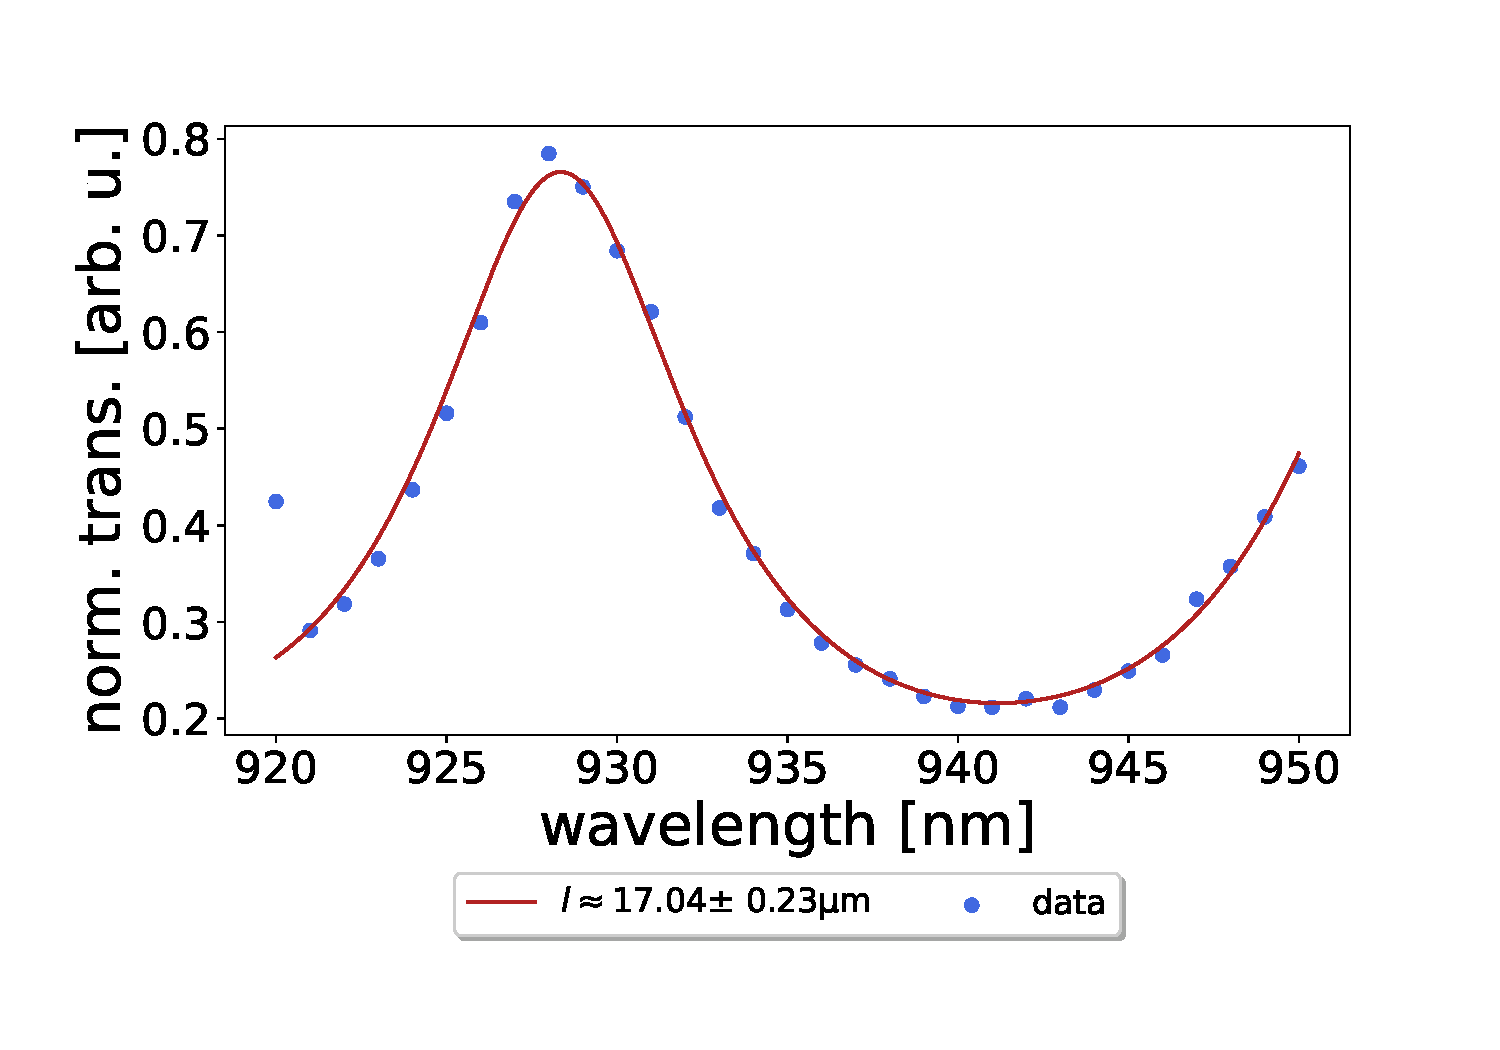
\includegraphics[width=\textwidth]{figures/results/double fano fits/30um_M3:M5_FSR_scan.pdf}
        \caption{}
        \label{fig:short_double_fano_FSR}
    \end{subfigure}
    \begin{subfigure}[b]{0.49\textwidth}
        \centering
        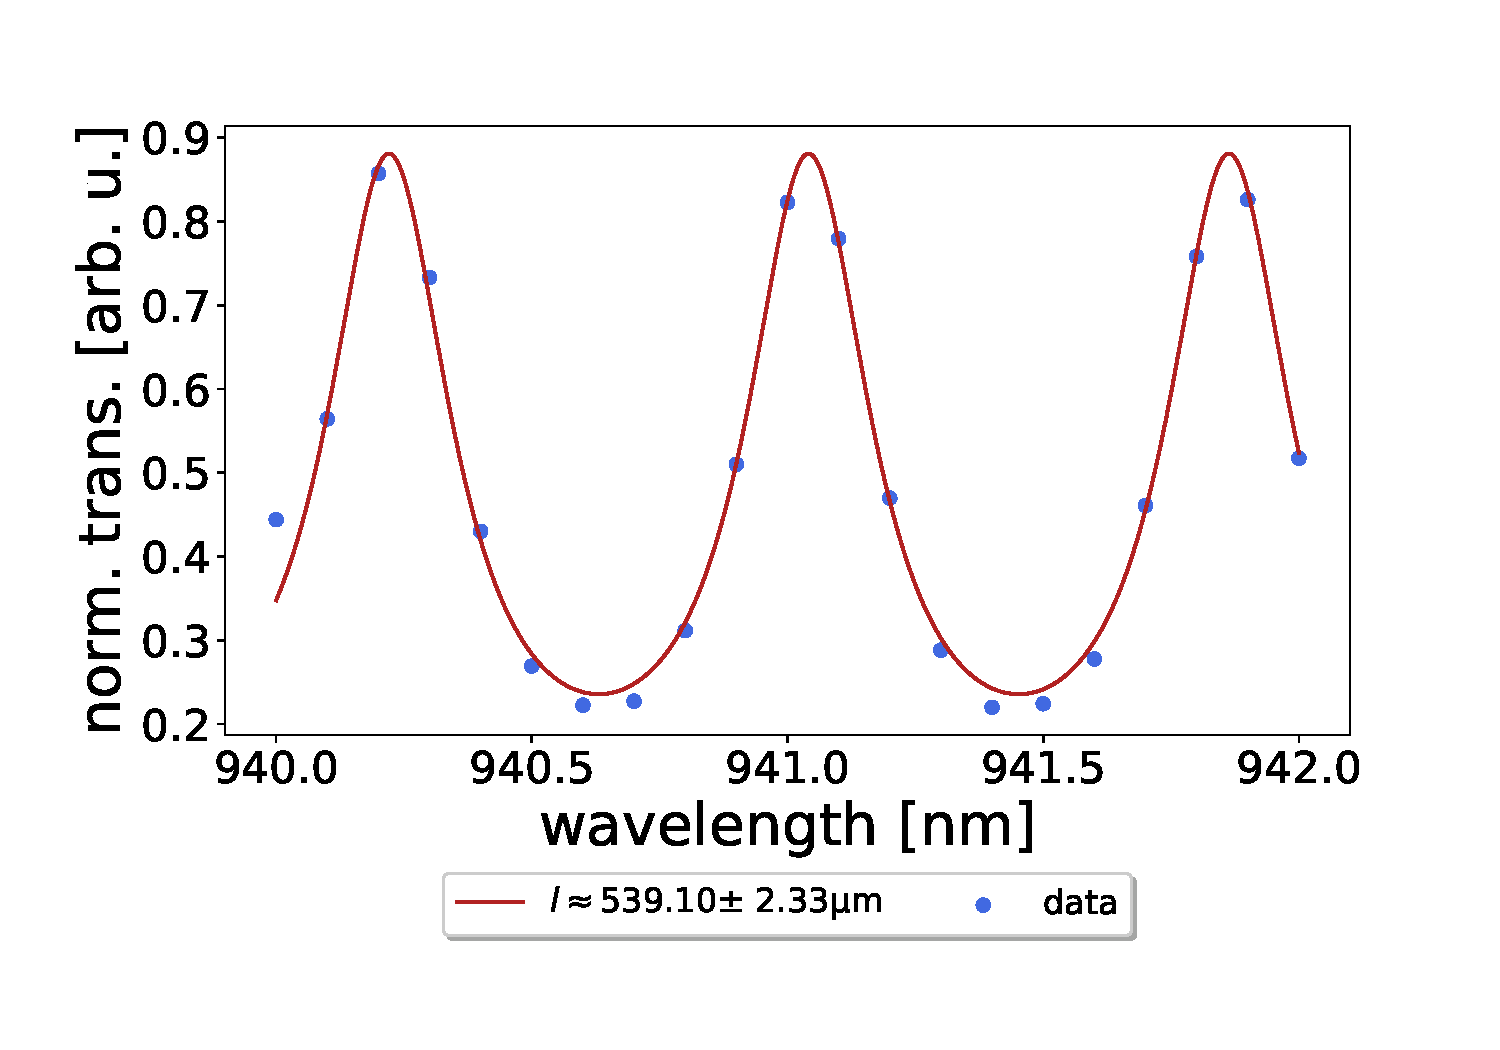
\includegraphics[width=\textwidth]{figures/results/double fano fits/550um_M3:M5_FSR_scan.pdf}
        \caption{}
        \label{fig:long_double_fano_FSR}
    \end{subfigure}
    \caption{}
    \label{fig:double_fano_fsr_scans}
\end{figure}

Figure \ref{fig:double_fano_trans_data} shows examples of resonance transmission spectra of the double Fano cavity. The examples are taken for length corresponding to the ones found from the off-resonance spectra shown in figure \ref{fig:double_fano_fsr_scans} above. The figures are depicted with each their corresponding least squares fits to the generalized Fano model shown in eq. (\ref{eq:general_fano_model}) in order to determine the linewidth (HWHM) of the profile. The errors of the linewidths are found from the error of each fit and are mainly used to determine the quality of the measurement. 

\begin{figure}[h!]
    \centering
    \begin{subfigure}[b]{0.49\textwidth}
        \centering
        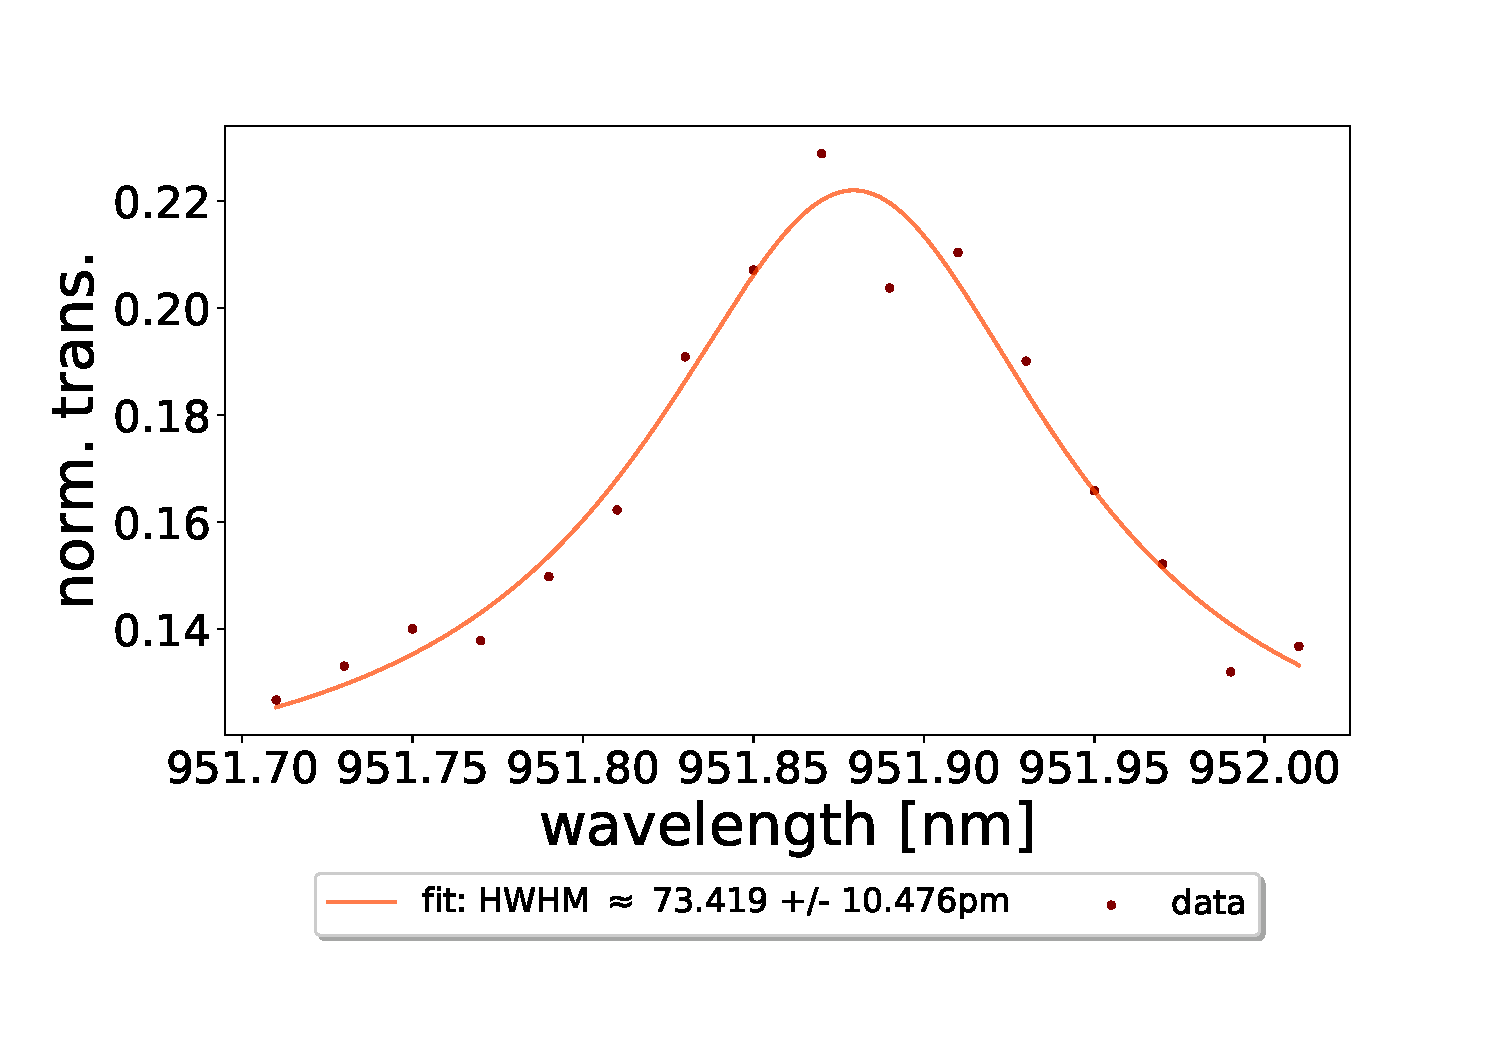
\includegraphics[width=\textwidth]{figures/results/double fano fits/30um_M3:M5_fit_4.pdf}
        \caption{}
        \label{fig:short_double_fano_trans}
    \end{subfigure}
    \begin{subfigure}[b]{0.49\textwidth}
        \centering
        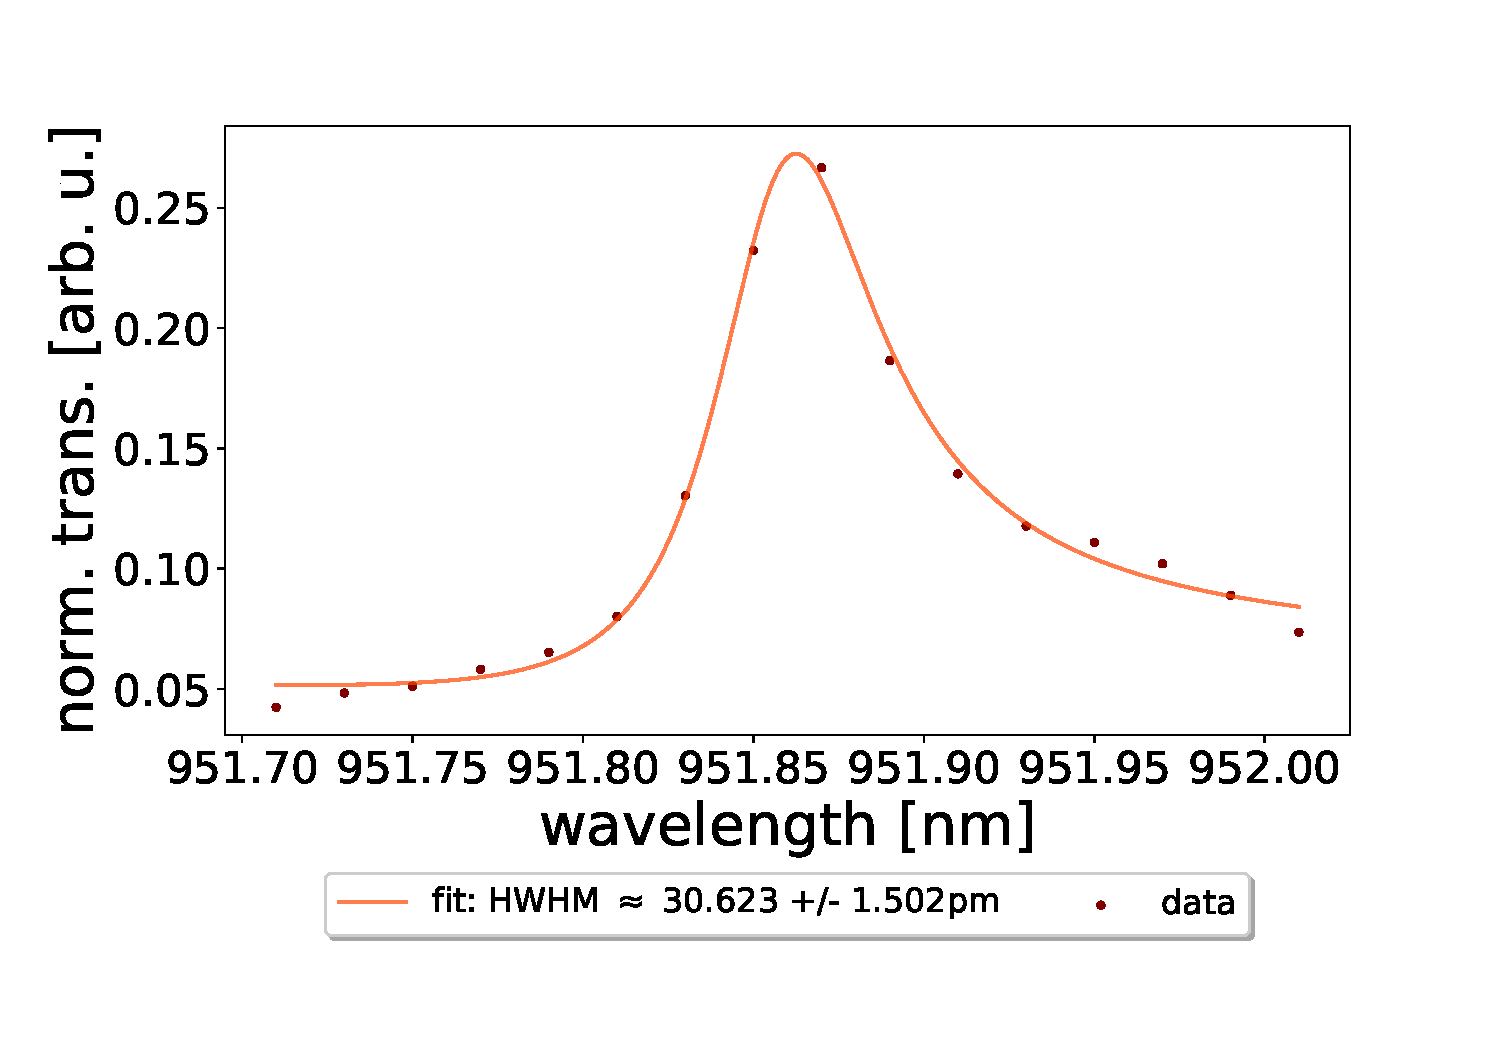
\includegraphics[width=\textwidth]{figures/results/double fano fits/550um_M3:M5_fit_1.pdf}
        \caption{}
        \label{fig:long_double_fano_trans}
    \end{subfigure}
    \caption{}
    \label{fig:double_fano_trans_data}
\end{figure}

Figure \ref{fig:HWHM_vs_l_double_fano_result} shows the average of results for the linewidths of a number of recorded spectra taken for cavity lengths in the approximate range $15 \mu m \leq l \leq 1000 \mu m$. The error of each data point depicted is determined as the standard deviation of all values found for the HWHM. The error in the x-direction, i.e. for the cavity lengths found from fits as the ones shown in figure \ref{fig:double_fano_fsr_scans} were of negligible size and are thus indicated rightly in the size of the data points themselves. The blue dashed line depict the analytical linewidth of a broadband cavity of losses similar to the double Fano cavity realized experimentally, the line is representative of eq. (\ref{eq:analytical_linewidth_broadband}). The orange dashed line similarly shows the analytical linewidth of the single Fano cavity calculated using eq. (\ref{eq:analytical_linewidth_single_fano}) for a cavity of similar losses. Lastly, the green dashed line indicate the analytical linewidth of the double Fano cavity transmission spectra comparable with the data points depicted. The black points are linewidths found by fitting double Fano transmission profiles simulated using eq. (\ref{eq:double_fano_transmission}) to the generalized Fano model in eq. (\ref{eq:general_fano_model}) for comparison.

It is seen that the analytical and simulated linewidths are strongly correlated, which indicates that both describe the transmission spectra well. This is also indicated in section \ref{sec:realizing_the_double_fano_model} where the realization of the double Fano model is shown to correlate well with the spectra produced. However,

\begin{figure}[h!]
    \centering
    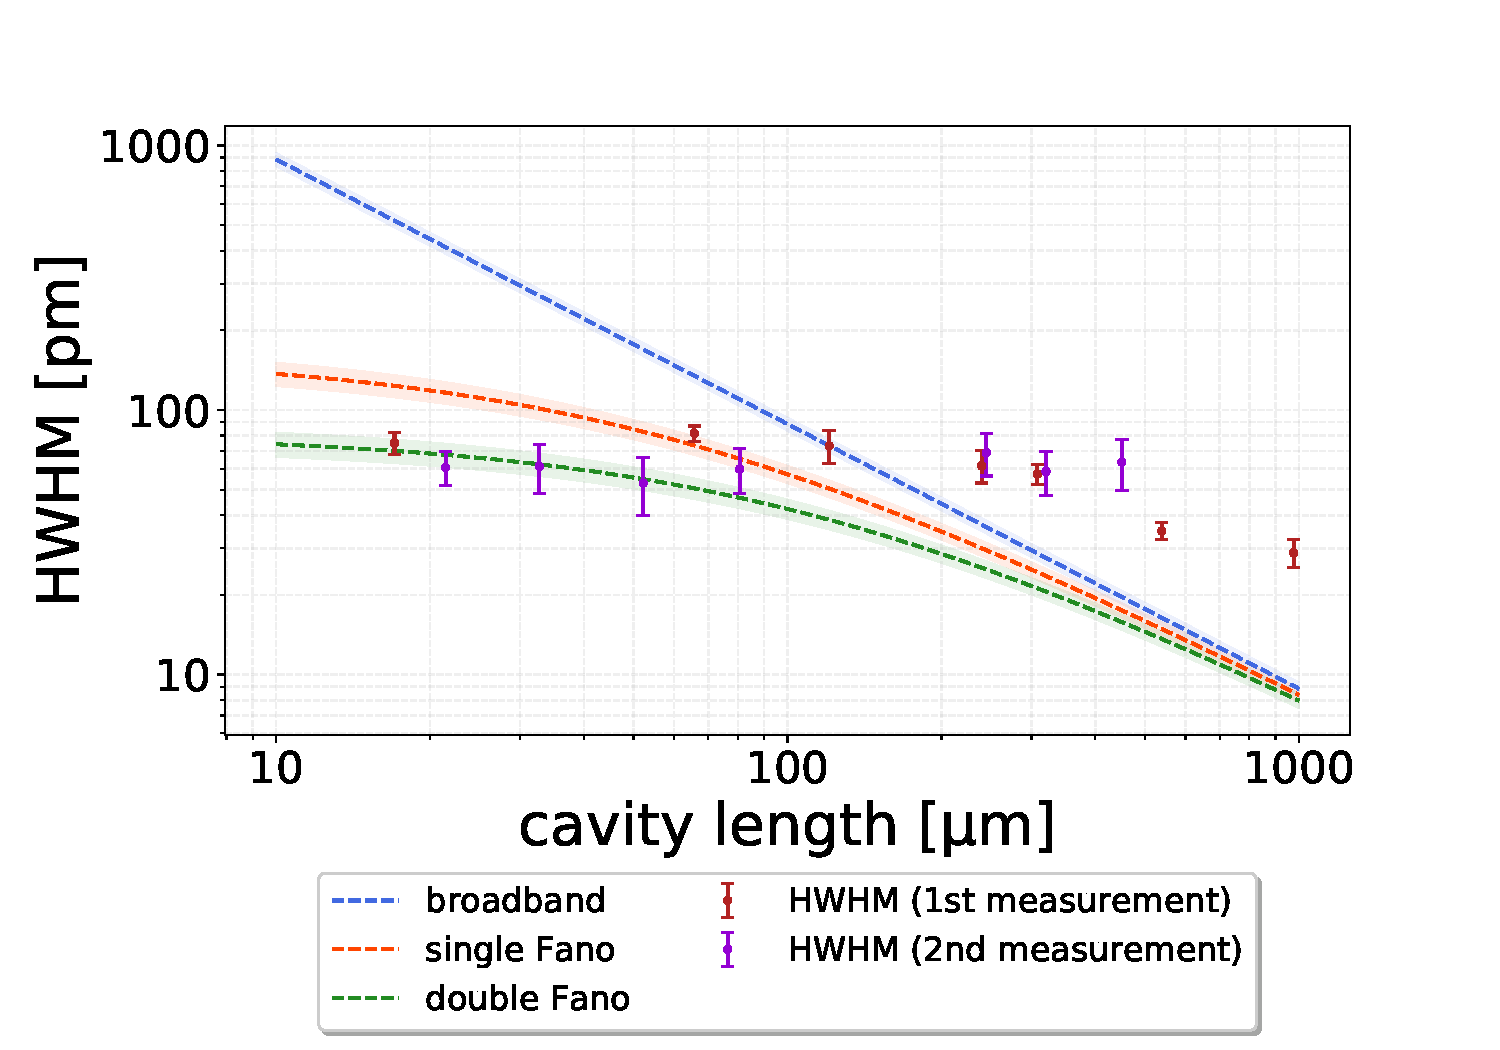
\includegraphics[width=0.7\textwidth]{figures/results/double fano fits/HWHM_vs_cavity_length_result.pdf}
    \caption{}
    \label{fig:HWHM_vs_l_double_fano_result}
\end{figure}

\subsection{Discussion}

\begin{figure}[h!]
    \centering
    \begin{subfigure}[b]{0.49\textwidth}
        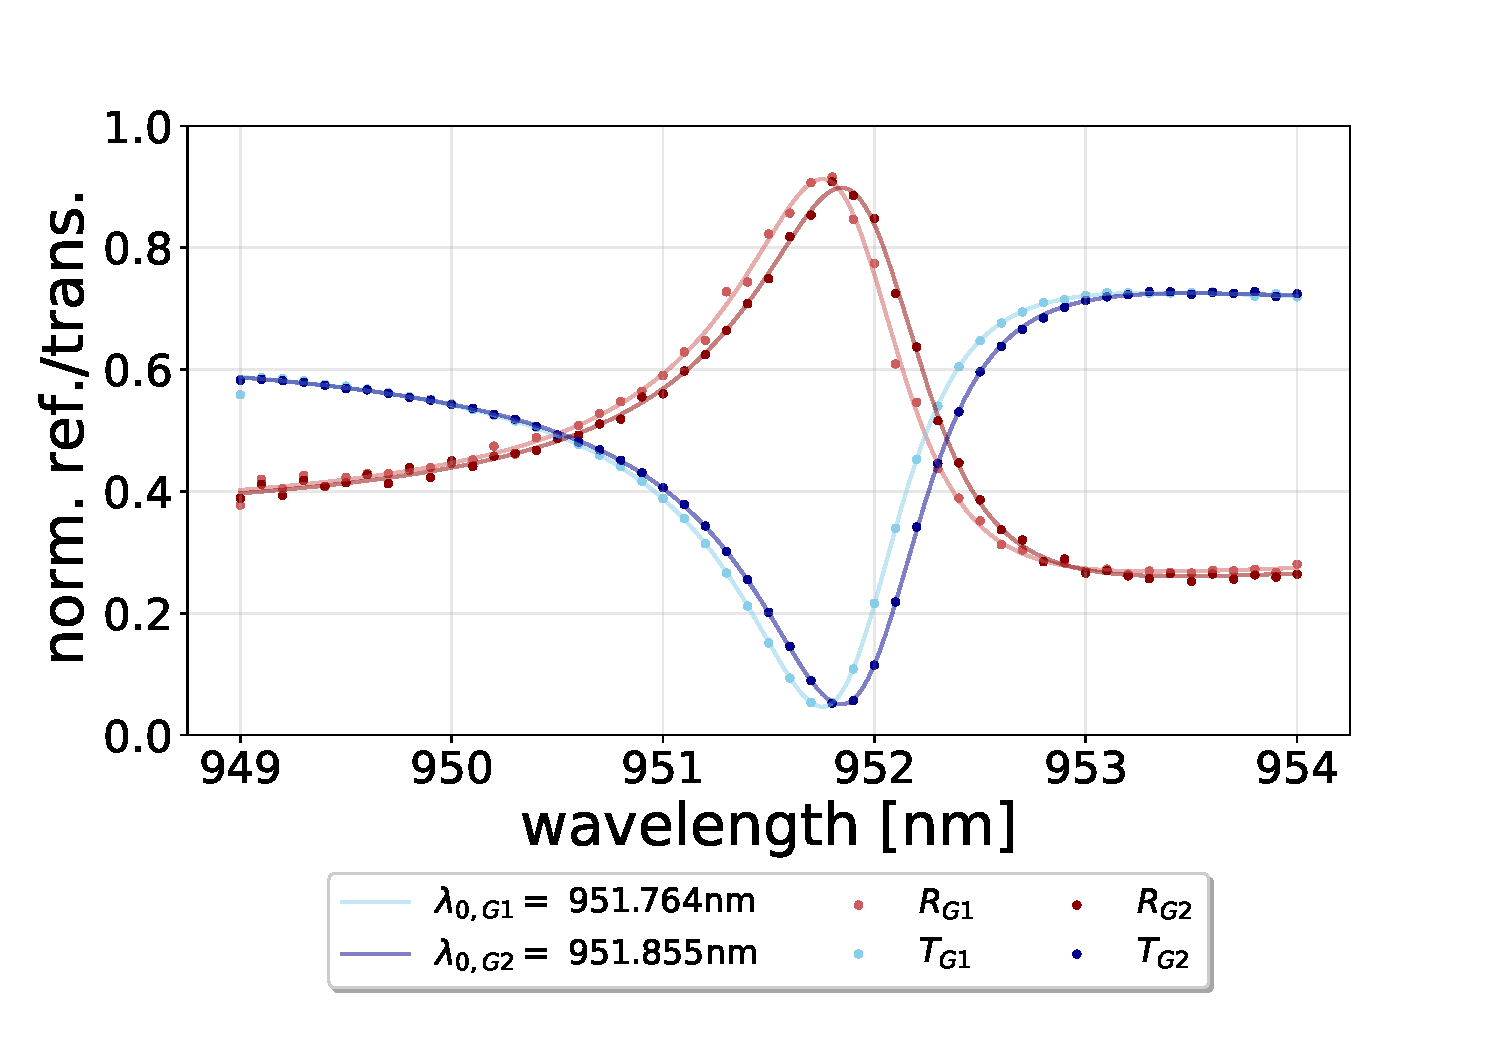
\includegraphics[width=\textwidth]{figures/results/M3:M5/M3:M5_initial_spectra.pdf}
        \caption{Individually measuret spectra of G1 and G2.}
        \label{}
    \end{subfigure}
    \begin{subfigure}[b]{0.49\textwidth}
        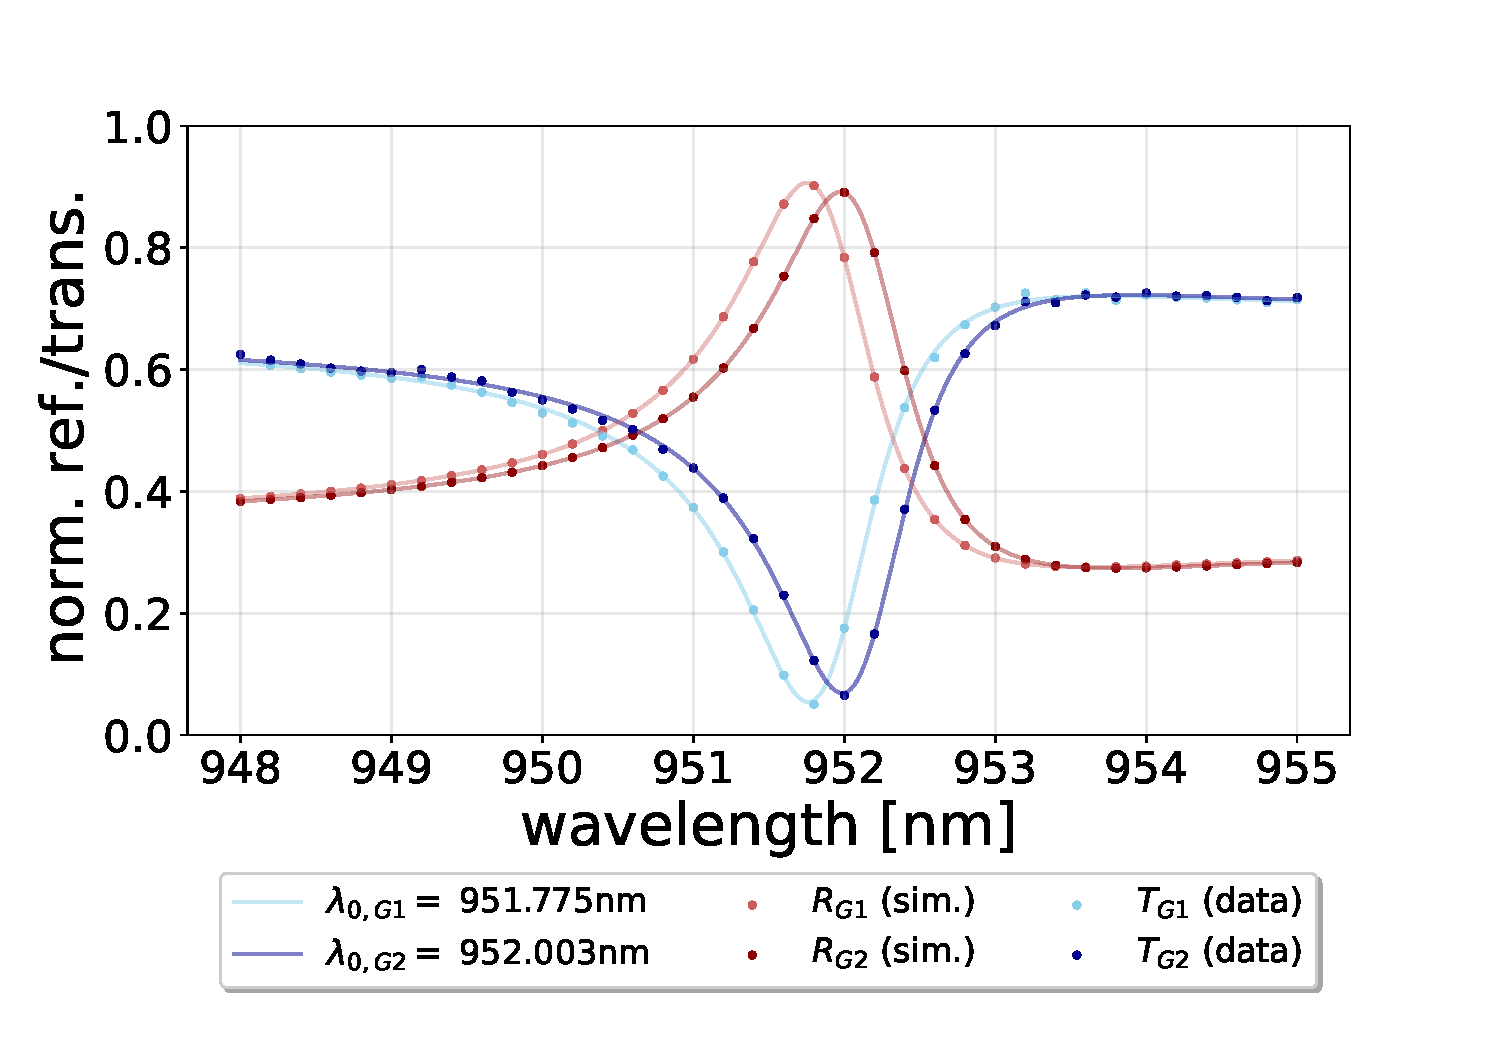
\includegraphics[width=\textwidth]{figures/results/M3:M5/M3:M5_spectra_at_measurement.pdf}
        \caption{Spectra of G1 and G2 in the double Fano config. i.e. where G2 is upside down.}
        \label{}
    \end{subfigure}
    \caption{}
    \label{}
\end{figure}

\begin{figure}[h!]
    \centering
    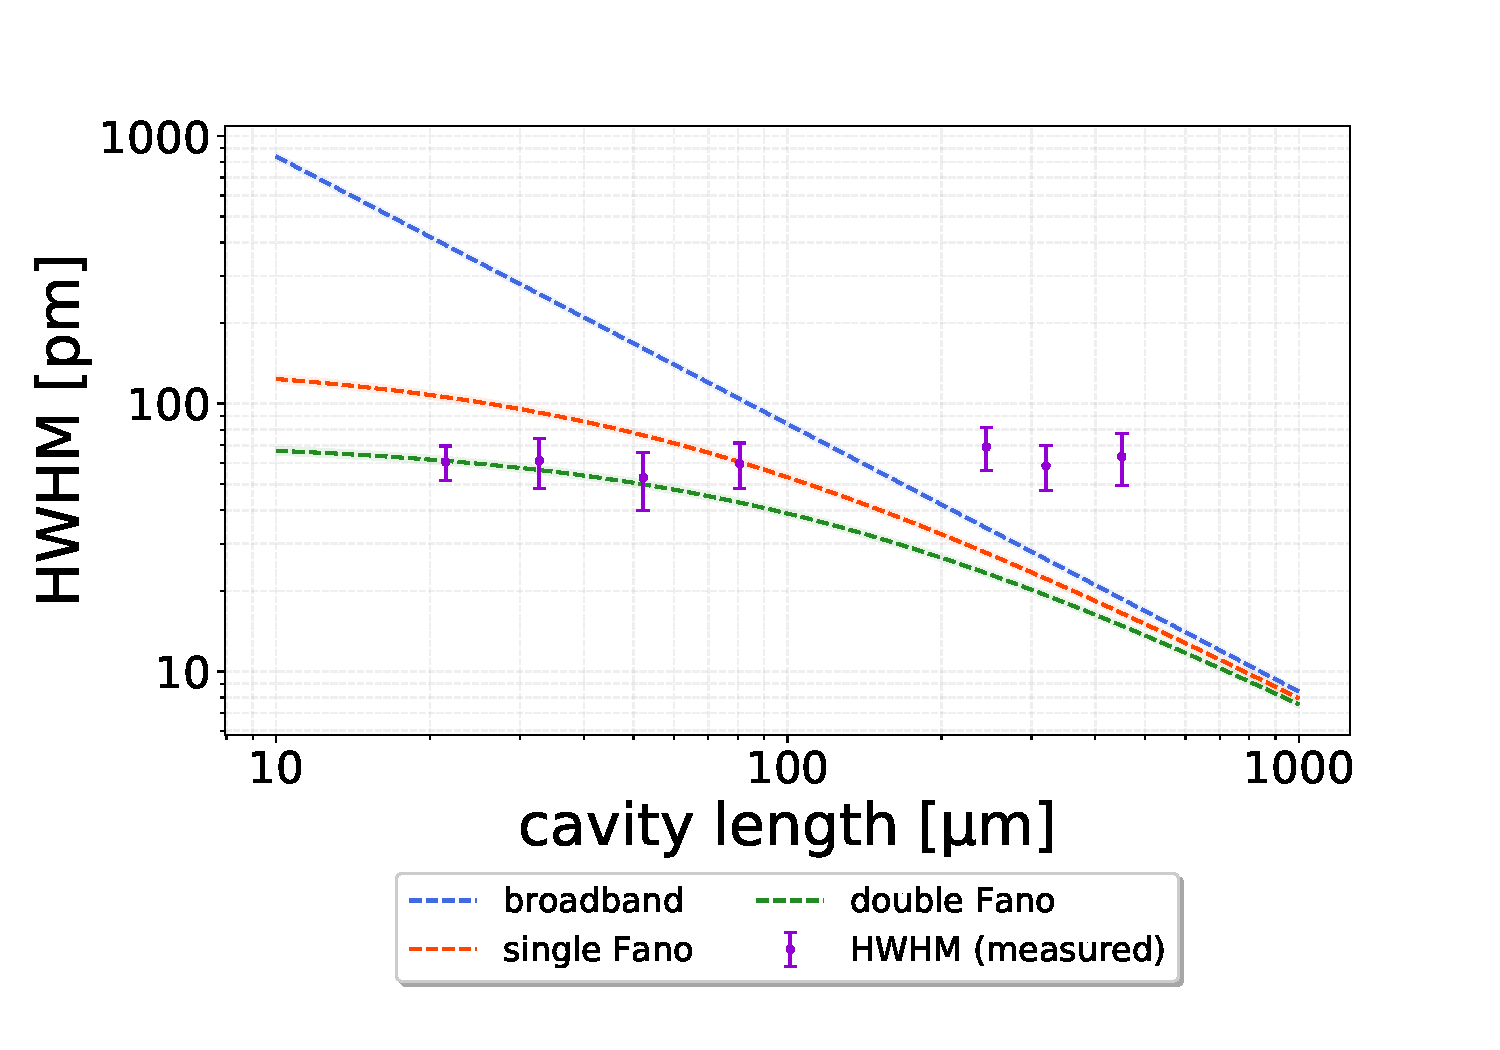
\includegraphics[width=0.7\textwidth]{figures/results/double fano fits/HWHM_vs_cavity_length_result_2nd_measurement_only.pdf}
    \caption{}
    \label{fig:HWHM_vs_l_double_fano_result_2nd}
\end{figure}

\begin{figure}[h!]
    \centering
    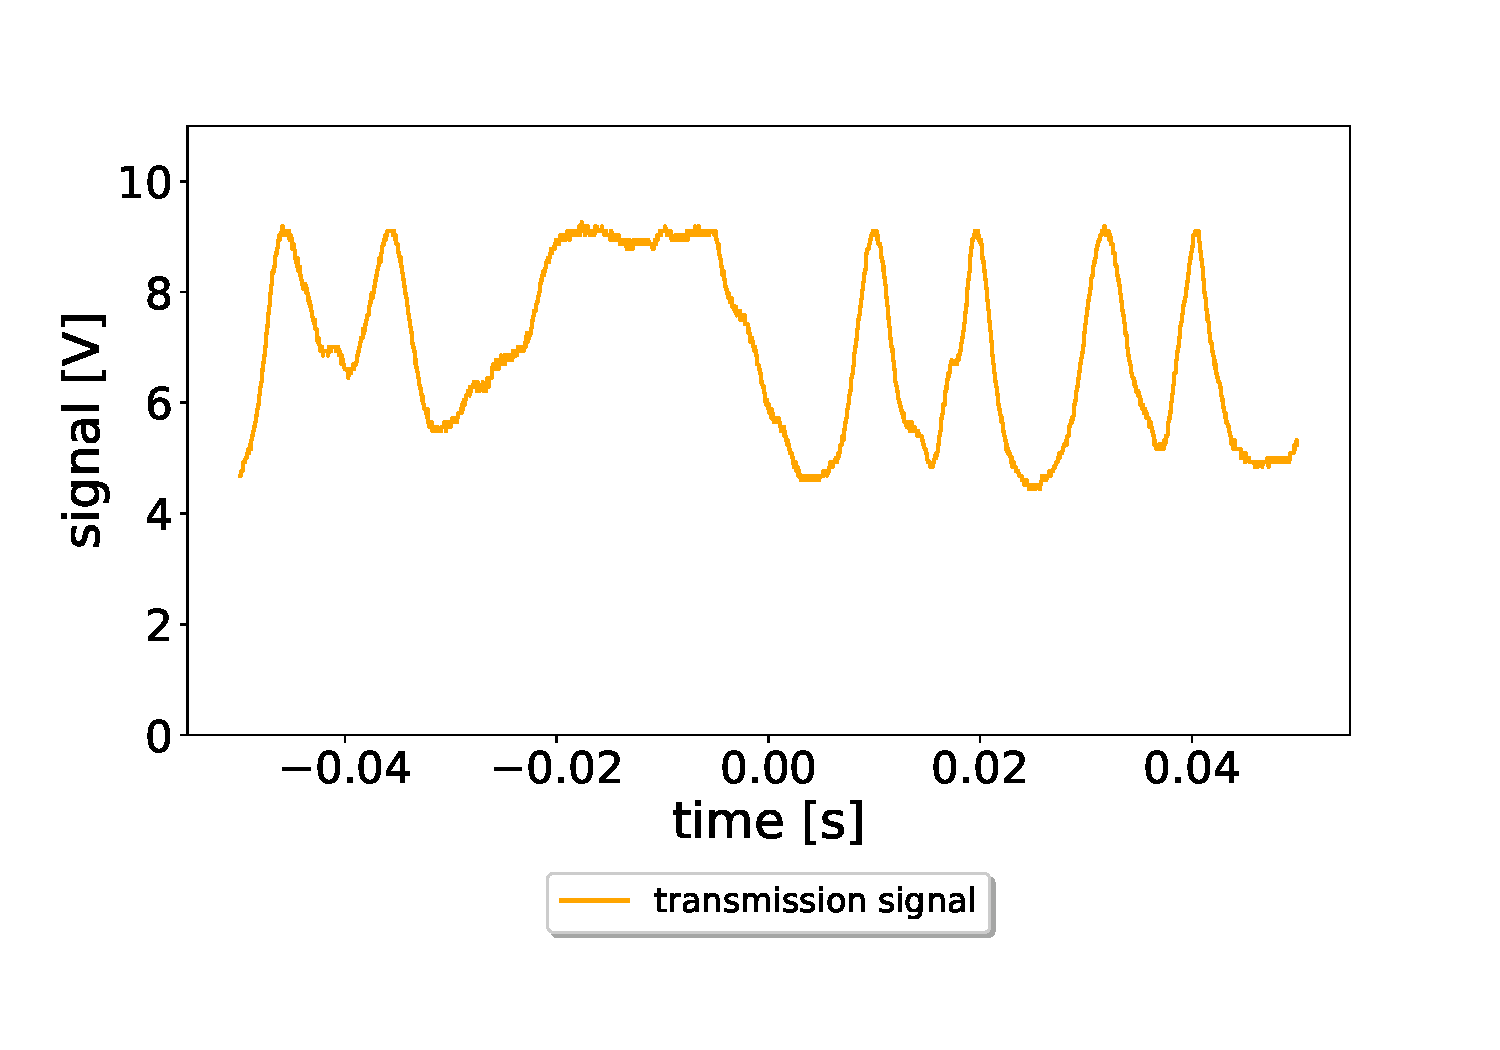
\includegraphics[width=0.7\textwidth]{figures/results/noise_on_resonance.pdf}
    \caption{}
    \label{fig:noise_on_resonance}
\end{figure}

Spacial drift of the piezo ring

Noise reduction - coupled/uncoupled mechanical/acoustic vibration (the plexi-glass box)

Broadening sources (especially for long cavities)

Improvements to the setup

The effect of flipping a fano mirror upside down

